% !TEX program = pdflatex
\documentclass[letterpaper,10pt,conference]{IEEEtran}
\IEEEoverridecommandlockouts

\usepackage{amsmath,amssymb,bm}
\usepackage{graphicx}
\usepackage{booktabs}
\usepackage{array}
\usepackage{url}
\usepackage{float}
\usepackage[section]{placeins}
\usepackage{xcolor}
\usepackage{listings}

\graphicspath{{images/}}
\newcommand{\vect}[1]{\bm{#1}}
\newcommand{\labstep}[1]{%
  \par\vspace{0.38\baselineskip}%
  \noindent\textbf{#1}\par\nobreak
  \vspace{0.10\baselineskip}%
}
\lstset{
  basicstyle=\ttfamily\fontsize{7}{9}\selectfont,
  breaklines=true,
  breakatwhitespace=false,
  columns=fullflexible,
  frame=single,
  framerule=0.35pt,
  framesep=4pt,
  framexleftmargin=3pt,
  framexrightmargin=3pt,
  framextopmargin=3pt,
  framexbottommargin=3pt,
  xleftmargin=0.25em,
  xrightmargin=0.25em,
  showstringspaces=false,
  keepspaces=true,
  numbers=none,
  aboveskip=0.45\baselineskip,
  belowskip=0.45\baselineskip,
  keywordstyle=\color{blue!60!black},
  commentstyle=\color{green!35!black},
  rulecolor=\color{black!65}
}
\setlength{\textfloatsep}{6pt plus 2pt minus 2pt}
\setlength{\floatsep}{6pt plus 2pt minus 2pt}
\setlength{\intextsep}{6pt plus 2pt minus 2pt}

\title{\LARGE \bf
Trajectory Optimization and Autonomous Drone Racing in Unity Simulation
}

\author{Wenqian Zhang\\
Student ID: 24020036087\\
VNAV Laboratory - Lab 4 Technical Report%
\thanks{Personal submission repository: \protect\url{https://github.com/OikawaZhang/vnav-personal-submissions}.}}

\begin{document}
\maketitle
\thispagestyle{empty}
\pagestyle{empty}

\begin{abstract}
This report presents the complete design, implementation, and validation procedure for Lab 4: Trajectory Optimization and Drone Racing. The work combines analytical trajectory optimization with a ROS-Unity autonomous-flight pipeline. The individual component derives single-segment minimum-velocity solutions for first-, second-, and third-degree polynomials, then studies an additional terminal-velocity constraint. The multi-segment component derives the constraint structure for minimum-snap and general minimum-$r$th-derivative trajectories. The programming component integrates the Lab 3 quadrotor controller, extracts the measured initial position from odometry, converts gate poses into position and continuous-yaw constraints, estimates segment times, solves polynomial minimum-snap problems, samples the resulting trajectories, and publishes complete desired states. The report records the commands, source files, implementation decisions, expected observations, and actual verification results in the order in which the experiment was performed. All 20 ROS packages compiled successfully, the first-gate hover was verified, and the baseline quadrotor completed the Unity course. Final speed optimization, the fastest-run video, and the corresponding final rosbag remain team submission items.
\end{abstract}

\section{Introduction and Objectives}
Autonomous drone racing requires trajectory planning, state estimation, feedback control, and simulator communication to operate as one closed-loop system. The vehicle must pass through gates with different positions and orientations while receiving a sufficiently smooth reference for stable tracking. Lab 4 therefore connects mathematical trajectory optimization to a complete ROS and Unity implementation.

The objectives of the experiment are: 1) to understand single- and multi-segment polynomial trajectory optimization; 2) to derive and apply minimum-snap optimization; 3) to integrate the controller developed in Lab 3; 4) to obtain the actual vehicle position from ROS odometry; 5) to convert gate poses into position and yaw constraints; 6) to sample an optimized trajectory and publish position, attitude, velocity, and acceleration references; and 7) to validate autonomous course completion in Unity. The final system must demonstrate that the waypoint publisher, trajectory generator, controller, TESSE bridge, and simulator form a functioning autonomous-flight loop.

\section{Background and Related Work}
\subsection{Polynomial Trajectory Representation}
Polynomial trajectories are widely used for quadrotor motion planning because their derivatives can be evaluated analytically and their boundary conditions can be written as linear constraints. For a segment of duration $T_i$, a scalar flat-output component is written as
\begin{equation}
p_i(t)=\sum_{n=0}^{N-1}c_{i,n}t^n,
\qquad 0\leq t\leq T_i.
\end{equation}
Position, velocity, acceleration, jerk, and snap follow by differentiating the same coefficient vector. Consequently, waypoint values and derivative conditions can be assembled into a quadratic program rather than enforced by an online nonlinear search. This representation is the mathematical basis of both the individual exercises and the \texttt{mav\_trajectory\_generation} implementation used in the lab.

\subsection{Differential Flatness and Minimum Snap}
A quadrotor is differentially flat with respect to position and yaw under the standard model, which means that the required attitude and control-related quantities can be reconstructed from a sufficiently smooth flat-output trajectory. Mellinger and Kumar used this property to formulate aggressive quadrotor flight as polynomial optimization and showed that minimizing the integral of squared snap produces references suitable for high-dynamic tracking~\cite{mellinger2011}. For a three-dimensional trajectory, the commonly used objective is
\begin{equation}
J_{\mathrm{snap}}=
\sum_{i=1}^{M}\int_0^{T_i}
\left\lVert\vect{p}_i^{(4)}(t)\right\rVert_2^2dt.
\end{equation}
Snap is the fourth derivative of position. Penalizing it discourages abrupt changes in lower-order motion quantities and therefore reduces discontinuities that would otherwise demand impulsive or rapidly changing control action. Minimum snap should not be confused with minimum time: the smoothness cost determines the shape of a trajectory for assigned segment durations, while the chosen durations determine how quickly that trajectory is executed.

\subsection{Piecewise Polynomials and Waypoint Continuity}
Real race courses require multiple segments because a single polynomial is inconvenient for enforcing a long sequence of gates. Adjacent segments must agree at shared waypoints. At minimum, position must be continuous; for a trackable quadrotor reference, velocity, acceleration, and typically higher derivatives must also remain compatible. Richter, Bry, and Roy developed an efficient formulation that separates constrained derivatives from free derivatives and solves for the latter to minimize the global trajectory cost~\cite{richter2016}. This structure explains the distinction used in Lab 4 between endpoint vertices created with \texttt{makeStartOrEnd} and intermediate vertices that contain only waypoint constraints.

Segment timing is equally important. Short durations produce faster reference motion but increase derivative magnitudes and tracking demand. The Lab 4 implementation first estimates durations from waypoint spacing and nominal velocity/acceleration parameters, then solves a linear polynomial problem. The parameters $v_{\max}$ and $a_{\max}$ therefore guide time allocation; they are not automatically guaranteed hard bounds on every optimized sample.

\subsection{Yaw Continuity and Angle Unwrapping}
Gate orientation is supplied as a quaternion, while the trajectory optimizer uses a scalar yaw angle. Because yaw is periodic, raw values near $-\pi$ and $\pi$ can appear far apart numerically even when the physical orientations are almost identical. The shortest signed angular increment is
\begin{equation}
\Delta\psi=operatorname{atan2}(\sin(\psi_i-\psi_{i-1}),
\cos(\psi_i-\psi_{i-1})).
\end{equation}
Accumulating this increment yields a continuous yaw sequence. Without unwrapping, the optimizer may command an unnecessary near-$2\pi$ rotation between two neighboring gates.

\subsection{Closed-Loop Tracking and Simulation}
Trajectory generation alone cannot fly the vehicle. The planner supplies feed-forward position, yaw, velocity, and acceleration references, while the Lab 3 feedback controller corrects the difference between desired and measured motion. Geometric quadrotor controllers formulate attitude directly on $\mathrm{SO}(3)$ and avoid the singularities associated with local attitude coordinates~\cite{lee2010}. Lab 4 reuses the previously tuned controller rather than redesigning it, allowing the experiment to focus on planning and integration.

ROS provides the message-passing layer for this closed loop. The waypoint publisher produces gate poses, the trajectory node produces desired states, the controller produces actuation commands, and the TESSE bridge exchanges state and control information with Unity. This modular arrangement makes each interface observable through topics and allows the static-hover test to validate the communication and controller chain before the full race trajectory is introduced.

\section{Deliverable 1: Single-Segment Optimization}
Consider
\begin{equation}
\min_{P(t)}J(P)=\int_0^1\left(P^{(1)}(t)\right)^2dt,
\quad P(0)=0,\quad P(1)=1.
\label{eq:minvel}
\end{equation}
Because $P(0)=0$, the constant coefficient is zero.

\subsection{First-Degree Polynomial}
For $P(t)=p_1t$, the terminal constraint gives $p_1=1$. Therefore, $P'(t)=1$ and
\begin{equation}
J(P)=\int_0^1 1^2dt=1,
\qquad \boxed{P^*(t)=t,\quad J^*=1.}
\end{equation}

\subsection{Second-Degree Polynomial}
Let
\begin{equation}
P(t)=p_1t+p_2t^2,
\qquad \vect{p}=\begin{bmatrix}p_1&p_2\end{bmatrix}^{T}.
\end{equation}
Since $P'(t)=p_1+2p_2t$,
\begin{align}
J(P)&=\int_0^1(p_1+2p_2t)^2dt\\
&=p_1^2+2p_1p_2+\frac{4}{3}p_2^2
=\vect{p}^{T}\vect{Q}\vect{p},
\end{align}
with
\begin{equation}
\boxed{\vect{Q}=\begin{bmatrix}1&1\\1&\frac{4}{3}\end{bmatrix}},
\quad
\boxed{\vect{A}=\begin{bmatrix}1&1\end{bmatrix}},
\quad
\boxed{\vect{b}=\begin{bmatrix}1\end{bmatrix}}.
\end{equation}
The constraint gives $p_1=1-p_2$, so
\begin{equation}
J(p_2)=1+\frac{1}{3}p_2^2.
\end{equation}
Thus, $p_2=0$, $p_1=1$, and
\begin{equation}
\boxed{\vect{p}^{*}=\begin{bmatrix}1&0\end{bmatrix}^{T},
\quad P^*(t)=t,\quad J^*=1.}
\end{equation}
Allowing a quadratic term does not reduce the optimal cost.

\subsection{Third-Degree Polynomial}
For
\begin{equation}
P(t)=p_1t+p_2t^2+p_3t^3,
\quad \vect{p}=\begin{bmatrix}p_1&p_2&p_3\end{bmatrix}^{T},
\end{equation}
the derivative basis is $[1,2t,3t^2]^T$. Integrating its outer product gives
\begin{equation}
\boxed{
\vect{Q}=\begin{bmatrix}
1&1&1\\
1&\frac{4}{3}&\frac{3}{2}\\
1&\frac{3}{2}&\frac{9}{5}
\end{bmatrix}},
\quad
\vect{A}=\begin{bmatrix}1&1&1\end{bmatrix},
\quad b=1.
\end{equation}
The equality-constrained QP is solved by the KKT system
\begin{equation}
\begin{bmatrix}
2\vect{Q}&\vect{A}^{T}\\
\vect{A}&0
\end{bmatrix}
\begin{bmatrix}\vect{p}\\\lambda\end{bmatrix}
=
\begin{bmatrix}\vect{0}\\b\end{bmatrix}.
\end{equation}
Substitution gives
\begin{equation}
\vect{p}^{*}=\begin{bmatrix}1&0&0\end{bmatrix}^{T},
\qquad \lambda^{*}=-2.
\end{equation}
The same result can be checked globally. The feasible polynomial $P(t)=t$ has cost one, and the Cauchy-Schwarz inequality yields
\begin{equation}
\int_0^1(P')^2dt\geq
\left(\int_0^1P'dt\right)^2=(P(1)-P(0))^2=1.
\end{equation}
Therefore this feasible polynomial is globally optimal:
\begin{equation}
\boxed{\vect{p}^{*}=\begin{bmatrix}1&0&0\end{bmatrix}^{T},
\quad P^*(t)=t,\quad J^*=1.}
\end{equation}
The Euler-Lagrange equation gives $\frac{d}{dt}(2P')=0$, or $P''=0$, which agrees with the linear optimum. Increasing polynomial degree alone cannot improve the result when only the two endpoint positions are constrained.

\subsection{Additional Terminal-Velocity Constraint}
Now impose
\begin{equation}
P(0)=0,\qquad P(1)=1,\qquad P'(1)=-2.
\end{equation}

For $P(t)=p_1t+p_2t^2$, the two terminal equations are
\begin{equation}
p_1+p_2=1,\qquad p_1+2p_2=-2.
\end{equation}
Equivalently,
\begin{equation}
\vect{A}_2=\begin{bmatrix}1&1\\1&2\end{bmatrix},
\qquad
\vect{b}_2=\begin{bmatrix}1\\-2\end{bmatrix}.
\end{equation}
Since $\vect{A}_2$ is nonsingular, the constraints uniquely give $p_1=4$ and $p_2=-3$. Hence
\begin{equation}
\boxed{P^*(t)=4t-3t^2,\qquad J^*=4.}
\end{equation}

For the cubic case, the constraints are
\begin{equation}
\underbrace{\begin{bmatrix}1&1&1\\1&2&3\end{bmatrix}}_{\vect{A}_3}
\begin{bmatrix}p_1\\p_2\\p_3\end{bmatrix}
=\underbrace{\begin{bmatrix}1\\-2\end{bmatrix}}_{\vect{b}_3}.
\end{equation}
Writing $p_3=c$ gives $p_1=4+c$ and $p_2=-3-2c$. Substitution into the cost yields
\begin{equation}
J(c)=4+c+\frac{2}{15}c^2.
\end{equation}
The stationary condition gives $c=-15/4$. Consequently,
\begin{equation}
\boxed{P^*(t)=\frac14t+\frac92t^2-\frac{15}{4}t^3,
\qquad J^*=\frac{17}{8}.}
\end{equation}
Unlike the original two-endpoint problem, the terminal-velocity constraint makes the quadratic solution more expensive. The cubic adds one degree of freedom and lowers the cost from $4$ to $17/8$ while satisfying all constraints.

\section{Deliverable 2: Multi-Segment Optimization}
\subsection{Minimum-Snap Trajectory over $k$ Segments}
For minimum snap, $r=4$, the Euler-Lagrange equation implies that every segment is a polynomial of degree $2r-1=7$~\cite{mittrajnotes}. Each segment therefore contains eight coefficients, and $k$ segments contain $8k$ unknown coefficients per spatial axis.

The constraints can be counted as follows. Each segment has a prescribed position at both endpoints, giving $2k$ waypoint equations. At the global start and end, velocity, acceleration, and jerk are fixed, giving six fixed-derivative equations. At each of the $k-1$ internal waypoints, derivatives of orders one through six must match between the adjacent polynomial pieces. These produce $6(k-1)$ free-derivative continuity equations. The count is
\begin{equation}
2k+6+6(k-1)=8k,
\end{equation}
which matches the number of polynomial coefficients. Equivalently, the derivatives of orders one through three at intermediate vertices may be treated as free optimization variables, while the variational optimality conditions enforce the remaining high-order continuity conditions.

\subsection{General Minimum-$r$th-Derivative Case}
For a cost of the form
\begin{equation}
J=\sum_{i=1}^{k}\int_0^{T_i}\left(P_i^{(r)}(t)\right)^2dt,
\end{equation}
each segment has degree $2r-1$ and therefore $2r$ coefficients. The complete trajectory has $2rk$ coefficients per axis. The corresponding equation count is
\begin{itemize}
\item $2k$ waypoint-position equations, one at each end of every segment;
\item $2(r-1)$ fixed derivatives at the global start and end, covering derivative orders $1$ through $r-1$;
\item $(2r-2)(k-1)$ continuity equations at internal waypoints, covering derivative orders $1$ through $2r-2$.
\end{itemize}
Their sum is
\begin{equation}
2k+2(r-1)+(2r-2)(k-1)=2rk.
\end{equation}
This general expression reduces to the minimum-snap count when $r=4$.

\subsection{Completion Summary and Personal Submission}
Table~\ref{tab:individual-completion} records the final status of the four requested individual items. All four are fully derived in this report.
\begin{table}[!htbp]
\caption{Completion of the Individual Deliverables}
\label{tab:individual-completion}
\centering
\footnotesize
\begin{tabular}{@{}p{0.35\columnwidth}p{0.55\columnwidth}@{}}
\toprule
Item & Completed result\\
\midrule
Cubic minimum velocity & $\vect{Q},\vect{A},b$ and KKT solution; $P^*(t)=t$, $J^*=1$\\
Constraint $P'(1)=-2$ & Quadratic: $4t-3t^2$, $J^*=4$; cubic: $\frac14t+\frac92t^2-\frac{15}{4}t^3$, $J^*=\frac{17}{8}$\\
$k$-segment minimum snap & $2k$ waypoint, $6(k-1)$ free-derivative continuity, and $6$ fixed-derivative equations\\
General derivative order $r$ & $2k$, $(2r-2)(k-1)$, and $2(r-1)$ equations; total $2rk$\\
\bottomrule
\end{tabular}
\end{table}
The typeset individual submission is associated with the repository listed in the title-page footnote.

\section{Experimental Environment and Architecture}
\subsection{Objectives and Software Environment}
The programming experiment integrates the Lab 3 controller, verifies first-gate hovering, reads the current UAV position, converts course gates to trajectory constraints, solves position and yaw trajectories, publishes desired states, and validates the closed loop in Unity. Table~\ref{tab:environment} summarizes the environment.

\begin{table}[!htbp]
\caption{Experimental Environment}
\label{tab:environment}
\centering
\footnotesize
\begin{tabular}{@{}p{0.31\columnwidth}p{0.60\columnwidth}@{}}
\toprule
Item & Configuration\\
\midrule
Operating system & Ubuntu 20.04\\
Virtual machine & Oracle VirtualBox\\
Middleware & ROS Noetic\\
Implementation & C++\\
Build system & Catkin\\
Simulator & Unity Lab 4\\
Trajectory library & \texttt{mav\_trajectory\_generation}\\
Workspace & \texttt{/home/oikawa/vnav\_ws}\\
\bottomrule
\end{tabular}
\end{table}

\subsection{Workspace Inspection and Package Roles}
Before modifying the source, the existing Lab 3 workspace was checked to avoid overwriting the controller:
\begin{lstlisting}[language=bash]
cd ~/vnav_ws
pwd
ls
ls src
\end{lstlisting}
The workspace contained \texttt{controller\_pkg}, \texttt{planner\_pkg}, \texttt{trajectory\_generation\_pkg}, \texttt{tesse-ros-bridge}, and \texttt{dependencies}. The controller computes flight commands; the planner publishes and processes gates; the trajectory package performs polynomial optimization and desired-state publication; the bridge connects ROS to Unity; and the dependency folder provides the required message and trajectory libraries. The presence of \texttt{src}, \texttt{build}, and \texttt{devel} confirmed that the Catkin workspace had already been configured.

Every new terminal used for ROS execution loaded the workspace environment:
\begin{lstlisting}[language=bash]
cd ~/vnav_ws
source devel/setup.bash
\end{lstlisting}
This command updates the shell environment so that \texttt{roslaunch} can locate the custom packages. A successful command normally returns without output.

\subsection{System Data Flow}
The data flow is
\begin{equation}
\text{Unity}\rightarrow\text{Bridge}\rightarrow\text{Current State}
\rightarrow\text{Planner/Optimizer}\rightarrow\text{Controller}\rightarrow\text{Unity}.
\end{equation}
The waypoint publisher sends a \texttt{geometry\_msgs/PoseArray} on \texttt{/desired\_traj\_vertices}. The trajectory node combines these poses with \texttt{/current\_state} odometry and publishes \texttt{/desired\_state}. The controller converts the desired and measured states into control commands, while the bridge transfers states and commands between ROS and the simulator.

\section{Detailed Experimental Design and Implementation}
\subsection{Controller Migration and Configuration}
\labstep{Objective and files}
Lab 4 reuses the low-level controller developed in Lab 3. The relevant files were the Lab 3 \texttt{traj\_tracking.launch}, the Lab 4 \texttt{traj\_following.launch}, and \texttt{static\_point\_test.launch}. The original gains were inspected with
\begin{lstlisting}[language=bash]
cat ~/vnav_ws/src/controller_pkg/launch/traj_tracking.launch
cat ~/vnav_ws/src/trajectory_generation_pkg/launch/traj_following.launch
cat ~/vnav_ws/src/planner_pkg/launch/static_point_test.launch
\end{lstlisting}
Both Lab 4 launch files were configured with
\begin{equation}
k_x=1,\qquad k_v=2,\qquad k_R=2,\qquad k_\omega=1.
\end{equation}
These gains respectively influence position, velocity, attitude, and angular-rate feedback. Keeping them consistent with Lab 3 prevents a controller known to work with one gain set from receiving a new trajectory under a different configuration.

\subsection{Part 0: First-Gate Hovering}
\labstep{Objective, file, and implementation}
The first test isolates the controller and communication chain from multi-segment optimization. The file \texttt{planner\_pkg/src/simple\_traj\_planner.cpp} was opened and the \texttt{trajCB()} callback was completed. The first pose is extracted using \texttt{traj\_msg.poses.front()}, copied into a \texttt{geometry\_msgs/Transform}, and inserted into a \texttt{MultiDOFJointTrajectoryPoint}. Zero velocity and acceleration request a stationary state at the target.
\begin{lstlisting}[language=C++]
const geometry_msgs::Pose& target_pose =
    traj_msg.poses.front();
trajectory_msgs::MultiDOFJointTrajectoryPoint desired_point;
geometry_msgs::Transform transform;
transform.translation.x = target_pose.position.x;
transform.translation.y = target_pose.position.y;
transform.translation.z = target_pose.position.z;
transform.rotation = target_pose.orientation;
desired_point.transforms.push_back(transform);
geometry_msgs::Twist zero_twist;
desired_point.velocities.push_back(zero_twist);
desired_point.accelerations.push_back(zero_twist);
desired_state_pub.publish(desired_point);
\end{lstlisting}
The same transform is broadcast from \texttt{world} to \texttt{desired\_pose}, making the reference available to ROS visualization and debugging tools.

\labstep{Operation and verification}
Three terminals were used:
\begin{lstlisting}[language=bash]
# Terminal 1
cd ~/vnav-builds/lab4 && ./lab4.x86_64
# Terminal 2
source ~/vnav_ws/devel/setup.bash
roslaunch tesse_ros_bridge tesse_quadrotor_bridge.launch
# Terminal 3
source ~/vnav_ws/devel/setup.bash
roslaunch planner_pkg static_point_test.launch
\end{lstlisting}
The expected behavior is flight toward the first gate followed by a near-stationary hover. The uploaded implementation contains the complete Part 0 logic, and the Unity observation in Fig.~\ref{fig:hover} verifies the resulting hover behavior.

\begin{figure}[!htbp]
\centering
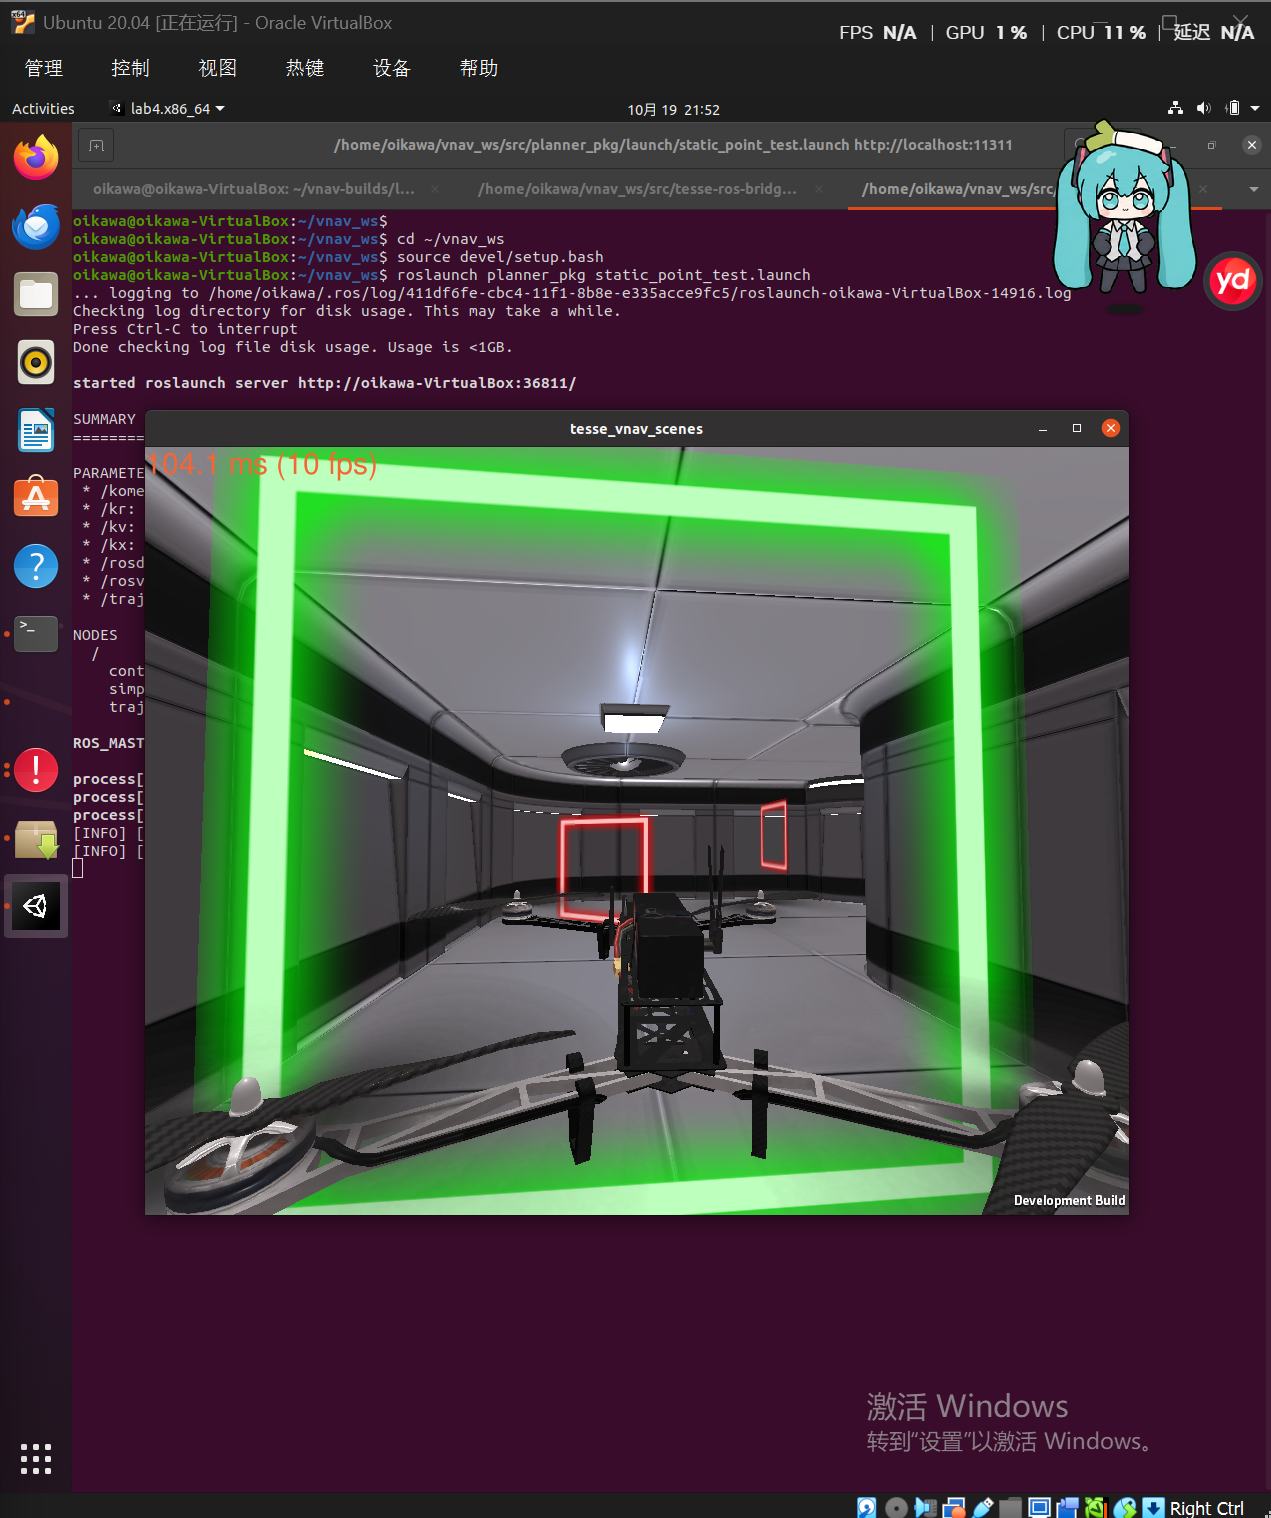
\includegraphics[width=0.94\columnwidth]{fig03_hover.png}
\caption{Quadrotor hovering at the first gate during the Part 0 test.}
\label{fig:hover}
\end{figure}

\subsection{Part 1.1: Current-State Acquisition}
\labstep{Objective and code}
A complete trajectory must start from the measured UAV position rather than from an assumed location. In \texttt{trajectory\_generation\_node.cpp}, the \texttt{onCurrentState()} callback converts odometry into the Eigen representation expected by the optimization library:
\begin{lstlisting}[language=C++]
x = Eigen::Vector3d(
    cur_state.pose.pose.position.x,
    cur_state.pose.pose.position.y,
    cur_state.pose.pose.position.z);
\end{lstlisting}
The vector $\vect{x}=[x\;y\;z]^T$ is then used by \texttt{start\_position.makeStartOrEnd(x,SNAP)}. This prevents a discontinuity between the physical vehicle position and the first point of the optimized trajectory.

\labstep{Verification}
The measured state can be inspected with
\begin{lstlisting}[language=bash]
rostopic echo -n 1 /current_state
\end{lstlisting}
The expected message contains the current simulated position under \texttt{pose.pose.position}. The source inspection confirmed correct extraction, and the successful closed-loop run confirms that the state was available to the trajectory node.

\subsection{Part 1.2: Multi-Segment Trajectory Generation}
\labstep{Waypoint input and dimensionality}
The provided \texttt{traj\_vertices\_publisher.cpp} reads gate position and orientation data and publishes \texttt{/desired\_traj\_vertices} as a \texttt{geometry\_msgs/PoseArray}. The topic can be checked using
\begin{lstlisting}[language=bash]
rostopic list | grep desired_traj_vertices
rostopic type /desired_traj_vertices
rostopic echo -n 1 /desired_traj_vertices
\end{lstlisting}
The expected type is \texttt{geometry\_msgs/PoseArray}, with one position and quaternion orientation for each gate. Position optimization uses $D=3$, whereas yaw is a separate one-dimensional problem:
\begin{lstlisting}[language=C++]
const int D = 3;
Vertex start_position(D), end_position(D);
Vertex::Vector vertices;
Vertex start_yaw(1), end_yaw(1);
Vertex::Vector yaw_vertices;
\end{lstlisting}

\labstep{Start, intermediate, and final constraints}
The measured position is used as the start vertex. For every gate, the pose position is converted to \texttt{Eigen::Vector3d}. Intermediate gates receive only a position constraint, allowing derivative values to be selected by the optimizer. The last gate uses \texttt{makeStartOrEnd}, which also establishes the required endpoint derivative conditions.
\begin{lstlisting}[language=C++]
start_position.makeStartOrEnd(x, SNAP);
vertices.push_back(start_position);
if (i == poseArray.poses.size() - 1) {
  end_position.makeStartOrEnd(position, SNAP);
  vertices.push_back(end_position);
} else {
  vertex.addConstraint(POSITION, position);
  vertices.push_back(vertex);
}
\end{lstlisting}

\labstep{Yaw extraction and unwrapping}
Gate orientation is originally represented as a quaternion. The scalar yaw is obtained with \texttt{tf::getYaw}. Direct subtraction is unsafe near $-\pi$ and $\pi$: for example, $179^\circ$ and $-179^\circ$ are physically close but numerically differ by $358^\circ$. The code therefore normalizes each yaw increment:
\begin{lstlisting}[language=C++]
double yaw = tf::getYaw(pose.orientation);
double yaw_diff = yaw - last_yaw;
yaw_diff = std::atan2(std::sin(yaw_diff),
                      std::cos(yaw_diff));
yaw = last_yaw + yaw_diff;
\end{lstlisting}
The final yaw receives an endpoint constraint; intermediate yaws receive \texttt{ORIENTATION} constraints. Figure~\ref{fig:constraints} shows the implemented position and yaw logic.

\begin{figure}[!htbp]
\centering
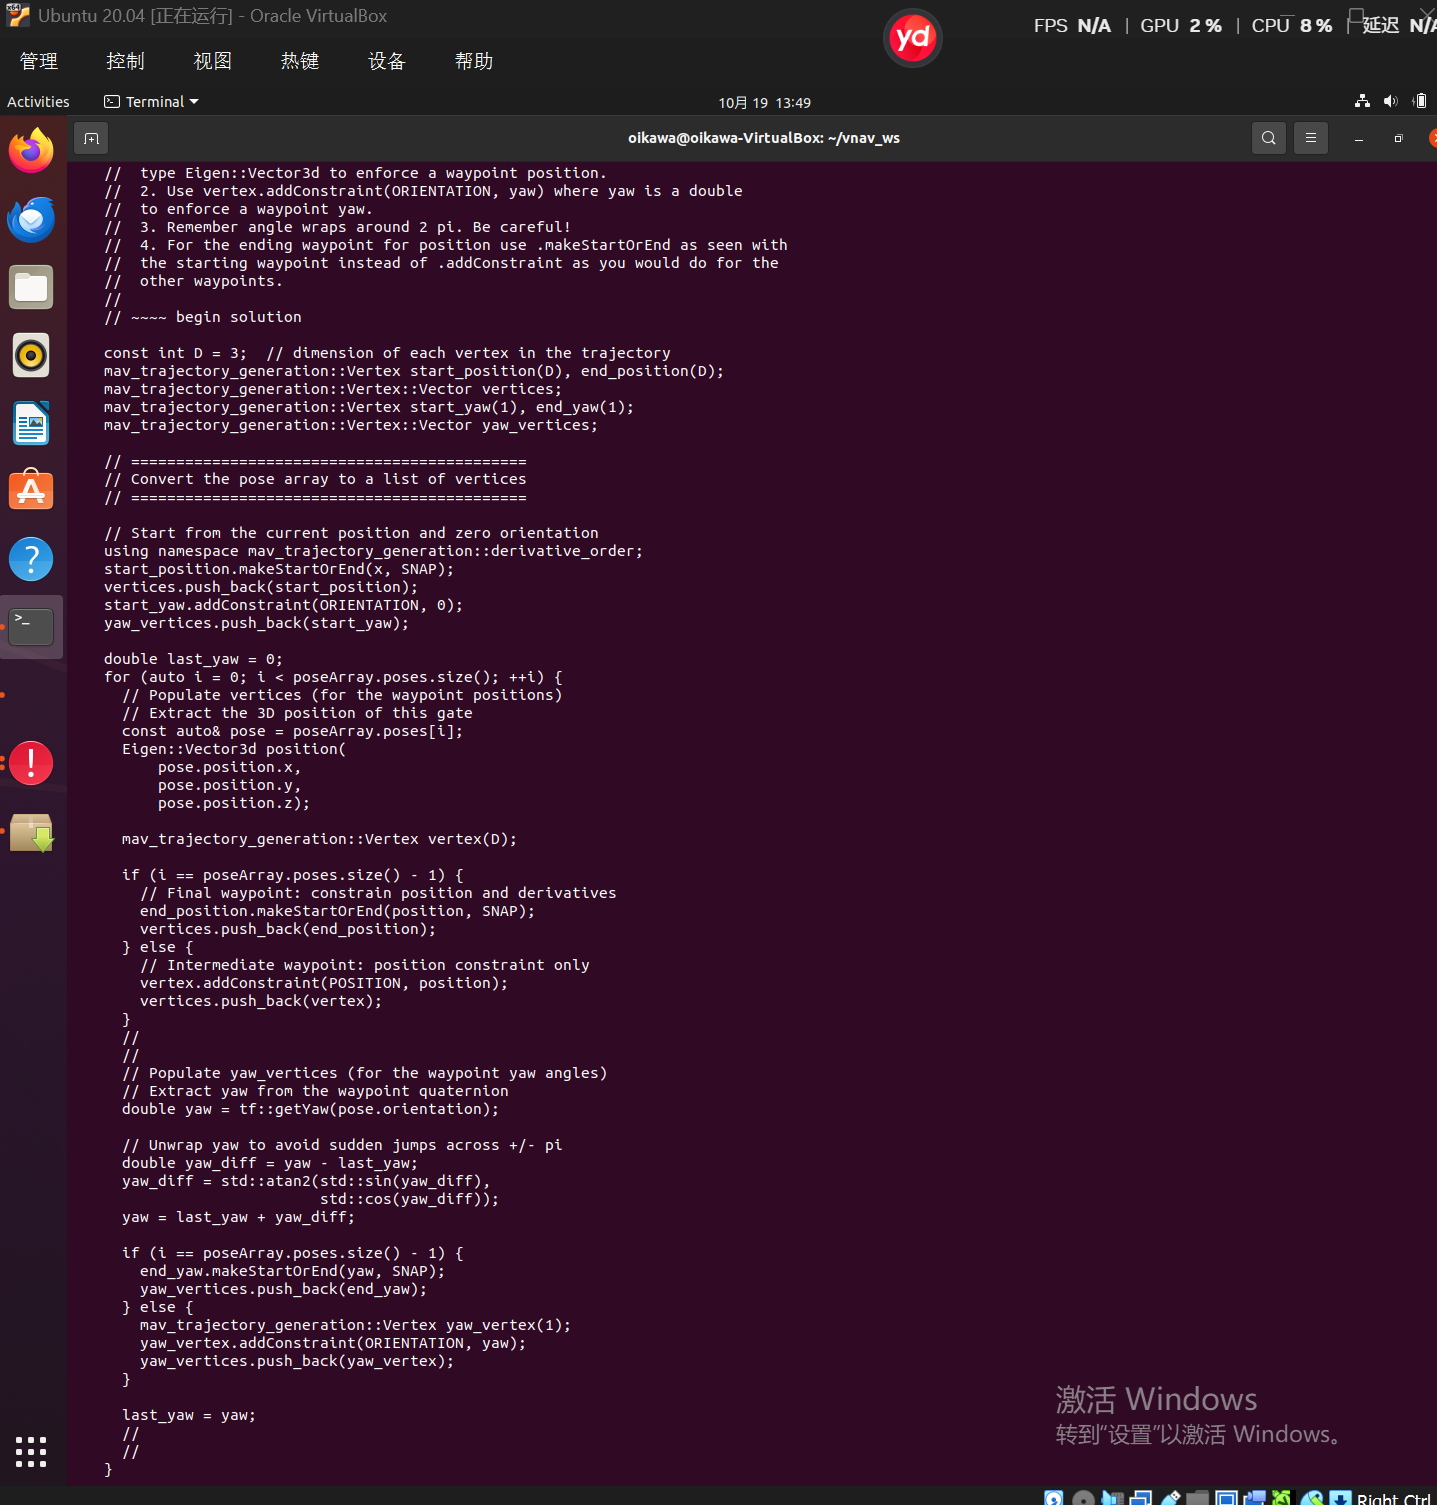
\includegraphics[width=0.94\columnwidth]{fig04_waypoint_code.png}
\caption{Implemented waypoint constraints and yaw-angle unwrapping.}
\label{fig:constraints}
\end{figure}

\labstep{Segment-time estimation}
Gate poses specify where the vehicle must travel, not how long each segment should take. Before polynomial optimization, segment durations are estimated using
\begin{lstlisting}[language=C++]
const double v_max = 8.0;
const double a_max = 4.0;
segment_times =
    estimateSegmentTimes(vertices, v_max, a_max);
\end{lstlisting}
The parameters guide time allocation based on waypoint spacing and dynamic scale. They should not be interpreted as strict measured bounds. For $M$ segments, the output is $\vect{T}=[T_1,\ldots,T_M]$ with positive entries. The source does not print these values, so no unobserved segment times are claimed.

\labstep{Minimum-snap solution and trajectory storage}
The implementation uses ten coefficients per segment, corresponding to a polynomial of maximum degree nine:
\begin{lstlisting}[language=C++]
const int N = 10;
PolynomialOptimization<N> opt(D);
opt.setupFromVertices(vertices, segment_times, SNAP);
opt.solveLinear();
PolynomialOptimization<N> yaw_opt(1);
yaw_opt.setupFromVertices(yaw_vertices,
                          segment_times, SNAP);
yaw_opt.solveLinear();
opt.getTrajectory(&trajectory);
yaw_opt.getTrajectory(&yaw_trajectory);
trajectoryStartTime = ros::Time::now();
\end{lstlisting}
Position and yaw are solved separately because their dimensions differ, but they share segment times so they remain synchronized during sampling. Minimum snap promotes high-order smoothness; it is not itself a minimum-time objective.

\subsection{Part 1.3: Trajectory Sampling and State Publication}
\labstep{Sampling time}
The optimized polynomial object is not sent directly to the controller. A ROS timer invokes \texttt{publishDesiredState()} at approximately 5 Hz. The elapsed time is computed relative to \texttt{trajectoryStartTime} and clamped to the valid range:
\begin{lstlisting}[language=C++]
double sampling_time =
    (ros::Time::now() - trajectoryStartTime).toSec();
if (sampling_time < 0.0) sampling_time = 0.0;
if (sampling_time > trajectory.getMaxTime())
  sampling_time = trajectory.getMaxTime();
next_point.time_from_start =
    ros::Duration(sampling_time);
\end{lstlisting}
Without this elapsed-time calculation, repeated sampling at zero would continually command the start state. Clamping also causes the final reference to be held after the planned duration.

\labstep{State evaluation and message construction}
At the same time instant, the position trajectory provides position, velocity, and acceleration, while the yaw trajectory provides orientation:
\begin{lstlisting}[language=C++]
Eigen::Vector3d des_position =
    trajectory.evaluate(sampling_time, POSITION);
Eigen::Vector3d des_velocity =
    trajectory.evaluate(sampling_time, VELOCITY);
Eigen::Vector3d des_accel =
    trajectory.evaluate(sampling_time, ACCELERATION);
Eigen::VectorXd des_orientation =
    yaw_trajectory.evaluate(sampling_time, ORIENTATION);
\end{lstlisting}
The position and quaternion are placed in \texttt{transforms}; the linear reference values are placed in \texttt{velocities} and \texttt{accelerations}; and the complete point is published with \texttt{desiredStatePub.publish(next\_point)}. Providing feed-forward velocity and acceleration gives the controller more information than a position-only reference.

\labstep{Topic verification}
The message type, rate, and fields can be checked with
\begin{lstlisting}[language=bash]
rostopic type /desired_state
rostopic hz /desired_state
rostopic echo -n 1 /desired_state
\end{lstlisting}
The expected type is \texttt{trajectory\_msgs/MultiDOFJointTrajectoryPoint}, and the observed rate should be close to the nominal 5 Hz subject to simulator load. The message should contain transforms, velocities, accelerations, and \texttt{time\_from\_start}. Figure~\ref{fig:progress} later shows that the sampled trajectory progressed to completion.

\section{Code Verification and Compilation}
\subsection{Source-Level Checks}
Compilation alone cannot prove that a commented placeholder has been implemented. Before building, the source was checked explicitly:
\begin{lstlisting}[language=bash]
cd ~/vnav_ws
grep -n "FILL IN HERE" \
  src/trajectory_generation_pkg/src/trajectory_generation_node.cpp
grep -n "desiredStatePub.publish" \
  src/trajectory_generation_pkg/src/trajectory_generation_node.cpp
\end{lstlisting}
The active source contained the publication call and no remaining placeholder in the required implementation. A separate backup file with a \texttt{.save} suffix is not part of the compiled target and should be excluded from the final repository.

\subsection{Workspace Build}
The complete workspace was rebuilt and sourced:
\begin{lstlisting}[language=bash]
cd ~/vnav_ws
catkin build
source devel/setup.bash
\end{lstlisting}
Figure~\ref{fig:buildprogress} documents progress across the 20-package workspace.

\begin{figure}[!htbp]
\centering
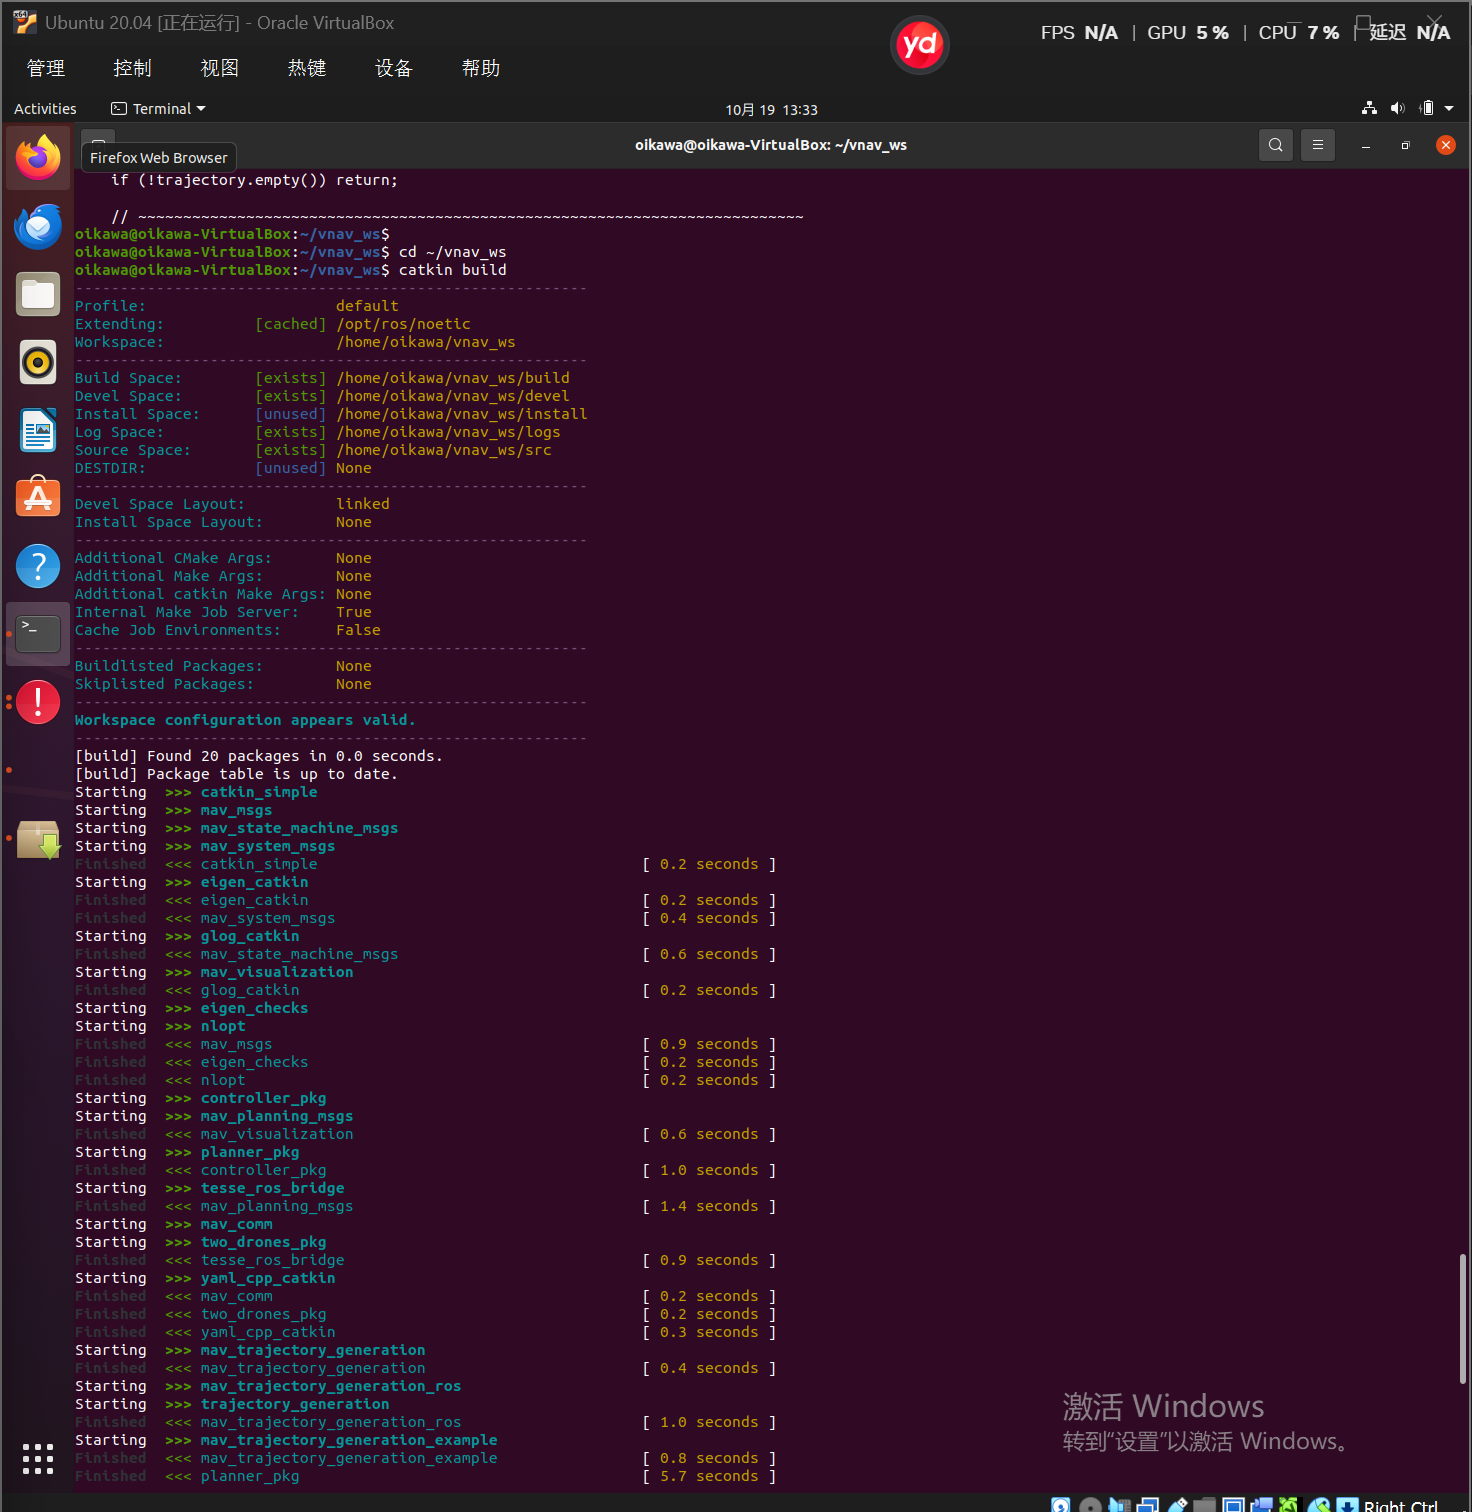
\includegraphics[width=0.94\columnwidth]{fig06_build_progress.png}
\caption{Catkin build progress across the 20-package ROS workspace.}
\label{fig:buildprogress}
\end{figure}

The compiler reported a non-blocking warning associated with a \texttt{size\_t} value printed using \texttt{\%d}. It should be changed to \texttt{\%zu} for type correctness, but it did not prevent executable generation. Figure~\ref{fig:warning} records the warning separately from the final success result.

\begin{figure}[!htbp]
\centering
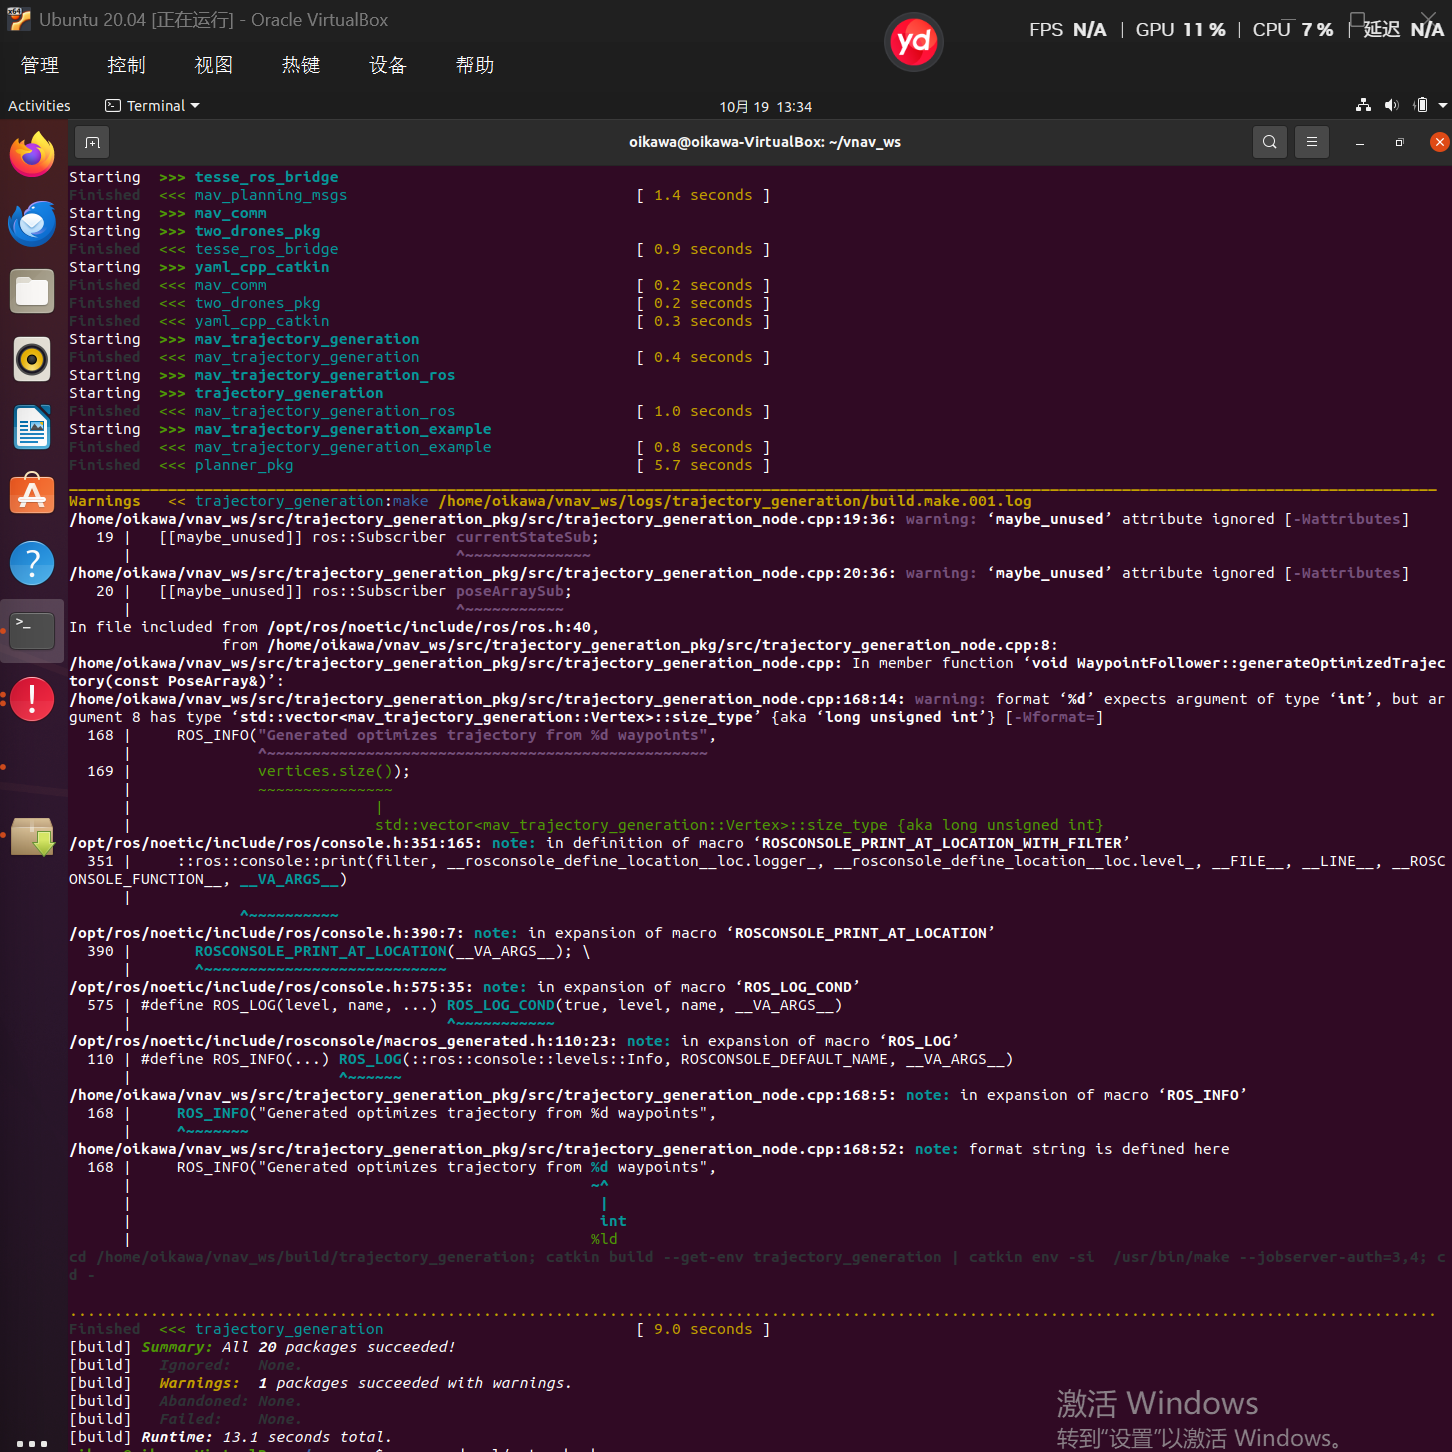
\includegraphics[width=0.94\columnwidth]{fig07_build_warning.png}
\caption{Non-blocking compiler warning and build summary.}
\label{fig:warning}
\end{figure}

After the final rebuild, all 20 packages succeeded, no package failed, and no package was abandoned. This verifies that the modified C++ code and dependencies formed a consistent Catkin workspace.

\begin{figure}[!htbp]
\centering
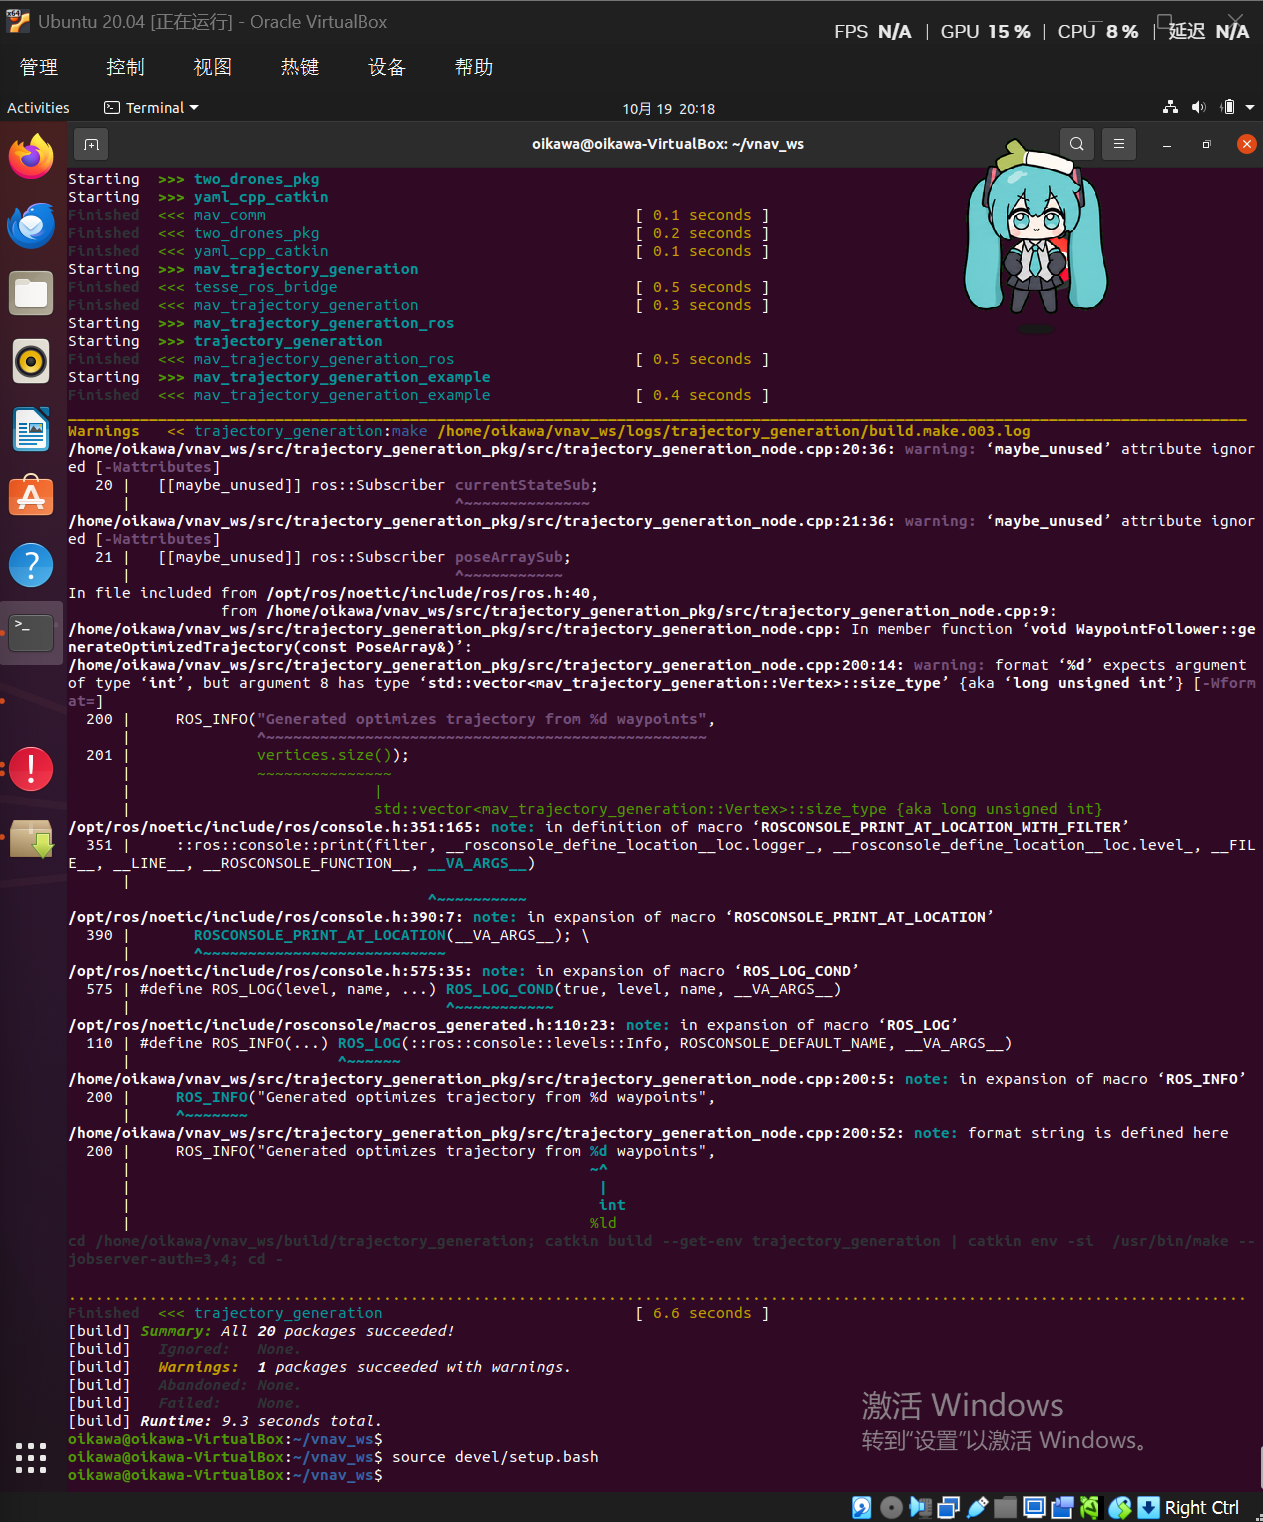
\includegraphics[width=0.94\columnwidth]{fig08_build_success.png}
\caption{Successful final compilation of the trajectory-generation system.}
\label{fig:buildsuccess}
\end{figure}

\section{Unity Setup and Full-System Execution}
\subsection{Simulator Installation and Launch}
The course simulator archive was downloaded, checked, extracted, and made executable:
\begin{lstlisting}[language=bash]
cd ~/Downloads
wget -c https://vnav.mit.edu/material/lab4.zip
ls -lh ~/Downloads/lab4.zip
unzip -t ~/Downloads/lab4.zip | tail -3
mkdir -p ~/vnav-builds
cd ~/vnav-builds
unzip -o ~/Downloads/lab4.zip
chmod +x ~/vnav-builds/lab4/lab4.x86_64
cd ~/vnav-builds/lab4
./lab4.x86_64
\end{lstlisting}
The integrity check guards against an incomplete download, while \texttt{chmod +x} provides the Linux executable permission. The simulator launched successfully from the expected directory, as shown in Fig.~\ref{fig:unitylaunch}.

\begin{figure}[!htbp]
\centering
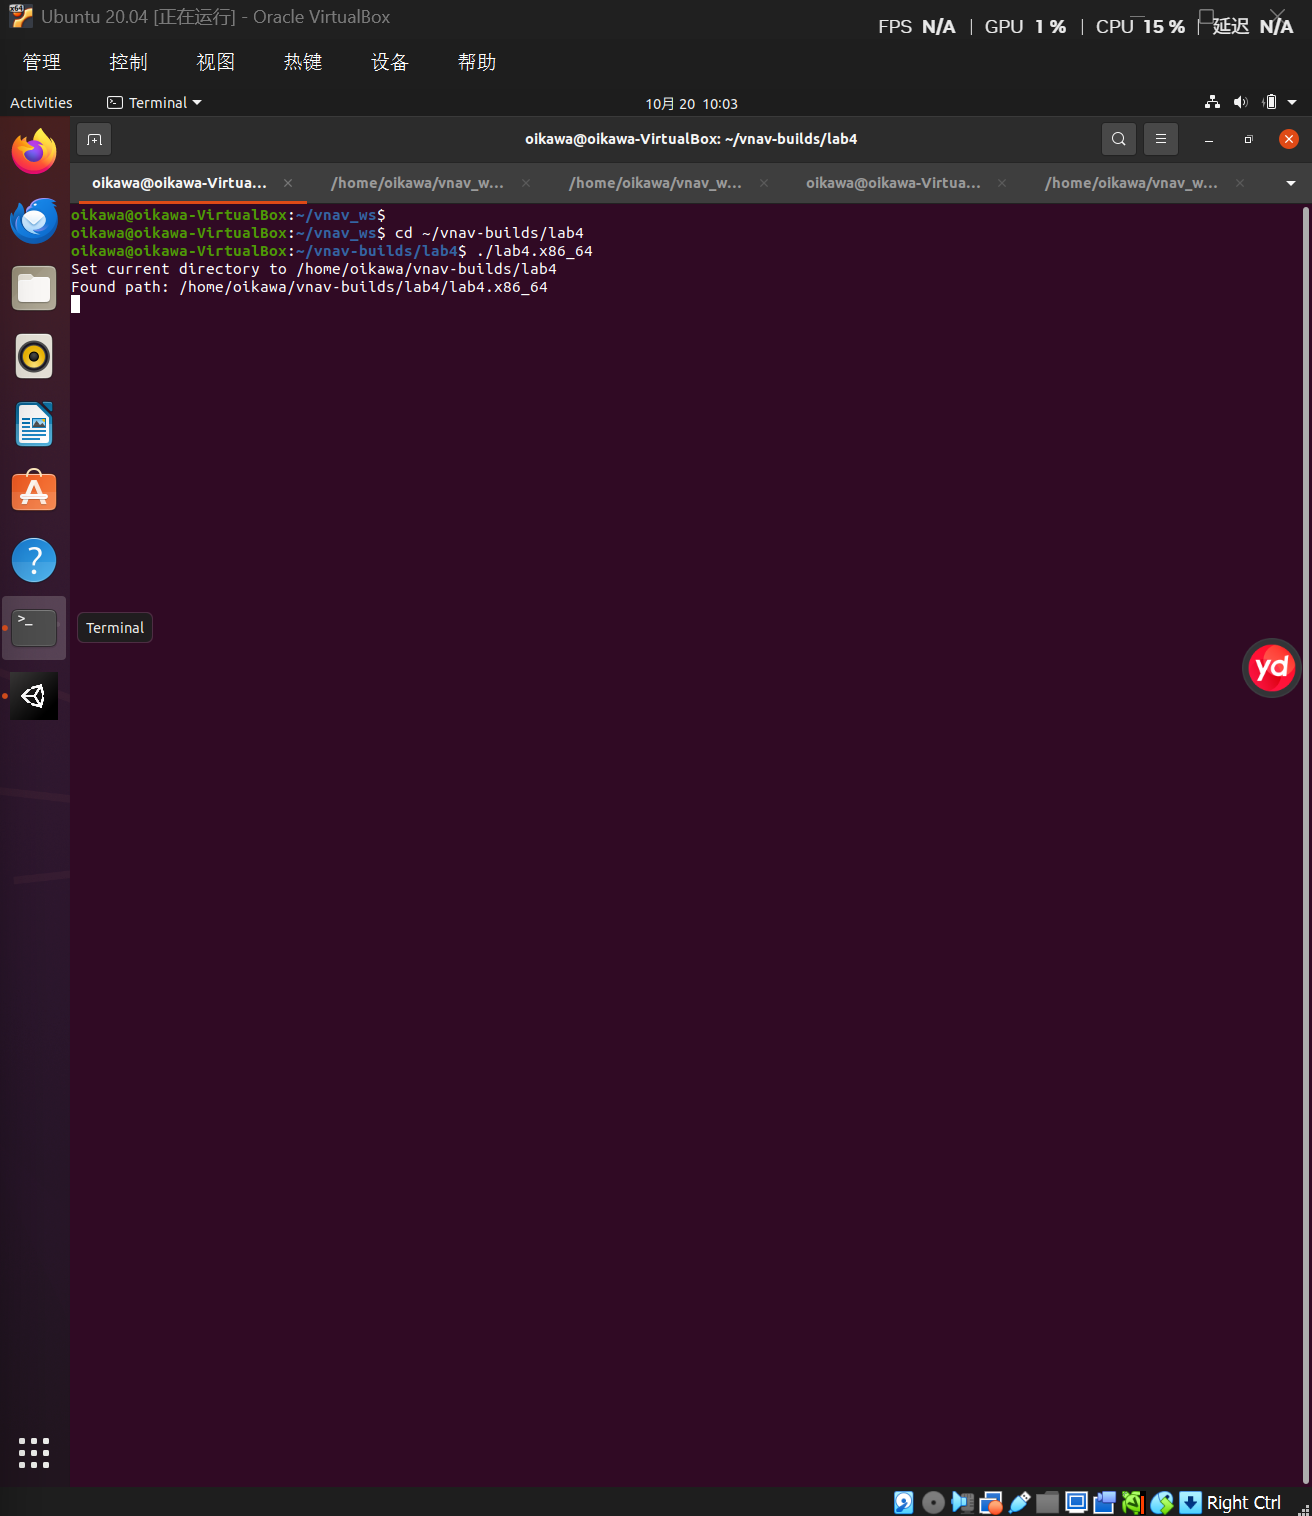
\includegraphics[width=0.94\columnwidth]{fig01_unity_launch.png}
\caption{Unity Lab 4 executable launched from the simulation directory.}
\label{fig:unitylaunch}
\end{figure}

The loaded scene contained the vehicle, course, and racing gates required for the experiment.

\begin{figure}[!htbp]
\centering
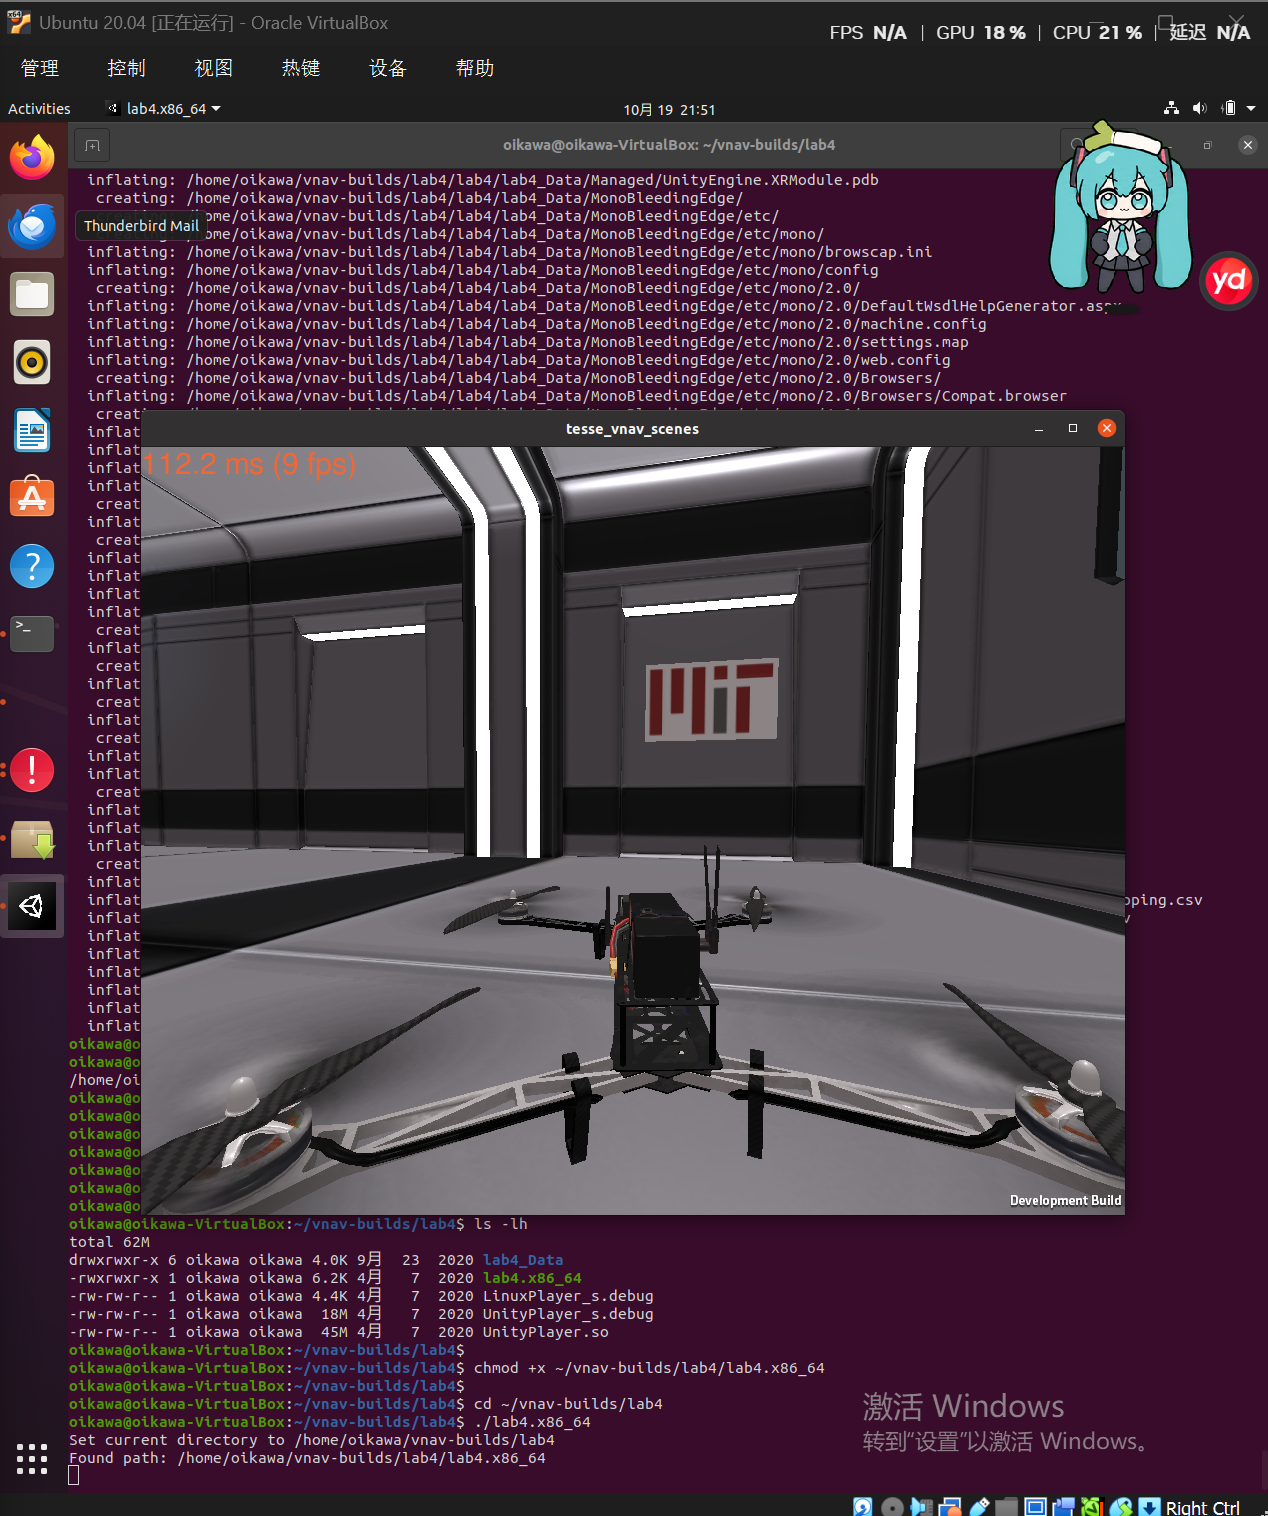
\includegraphics[width=0.94\columnwidth]{fig09_unity_scene.png}
\caption{Unity drone-racing environment before trajectory execution.}
\label{fig:scene}
\end{figure}

\subsection{Bridge Startup}
In a second terminal, the workspace was sourced and the TESSE bridge was launched:
\begin{lstlisting}[language=bash]
cd ~/vnav_ws
source devel/setup.bash
roslaunch tesse_ros_bridge \
  tesse_quadrotor_bridge.launch
\end{lstlisting}
The bridge makes Unity state available to ROS and forwards controller outputs to the simulator. Figure~\ref{fig:bridge} records the bridge startup and communication configuration.

\begin{figure}[!htbp]
\centering
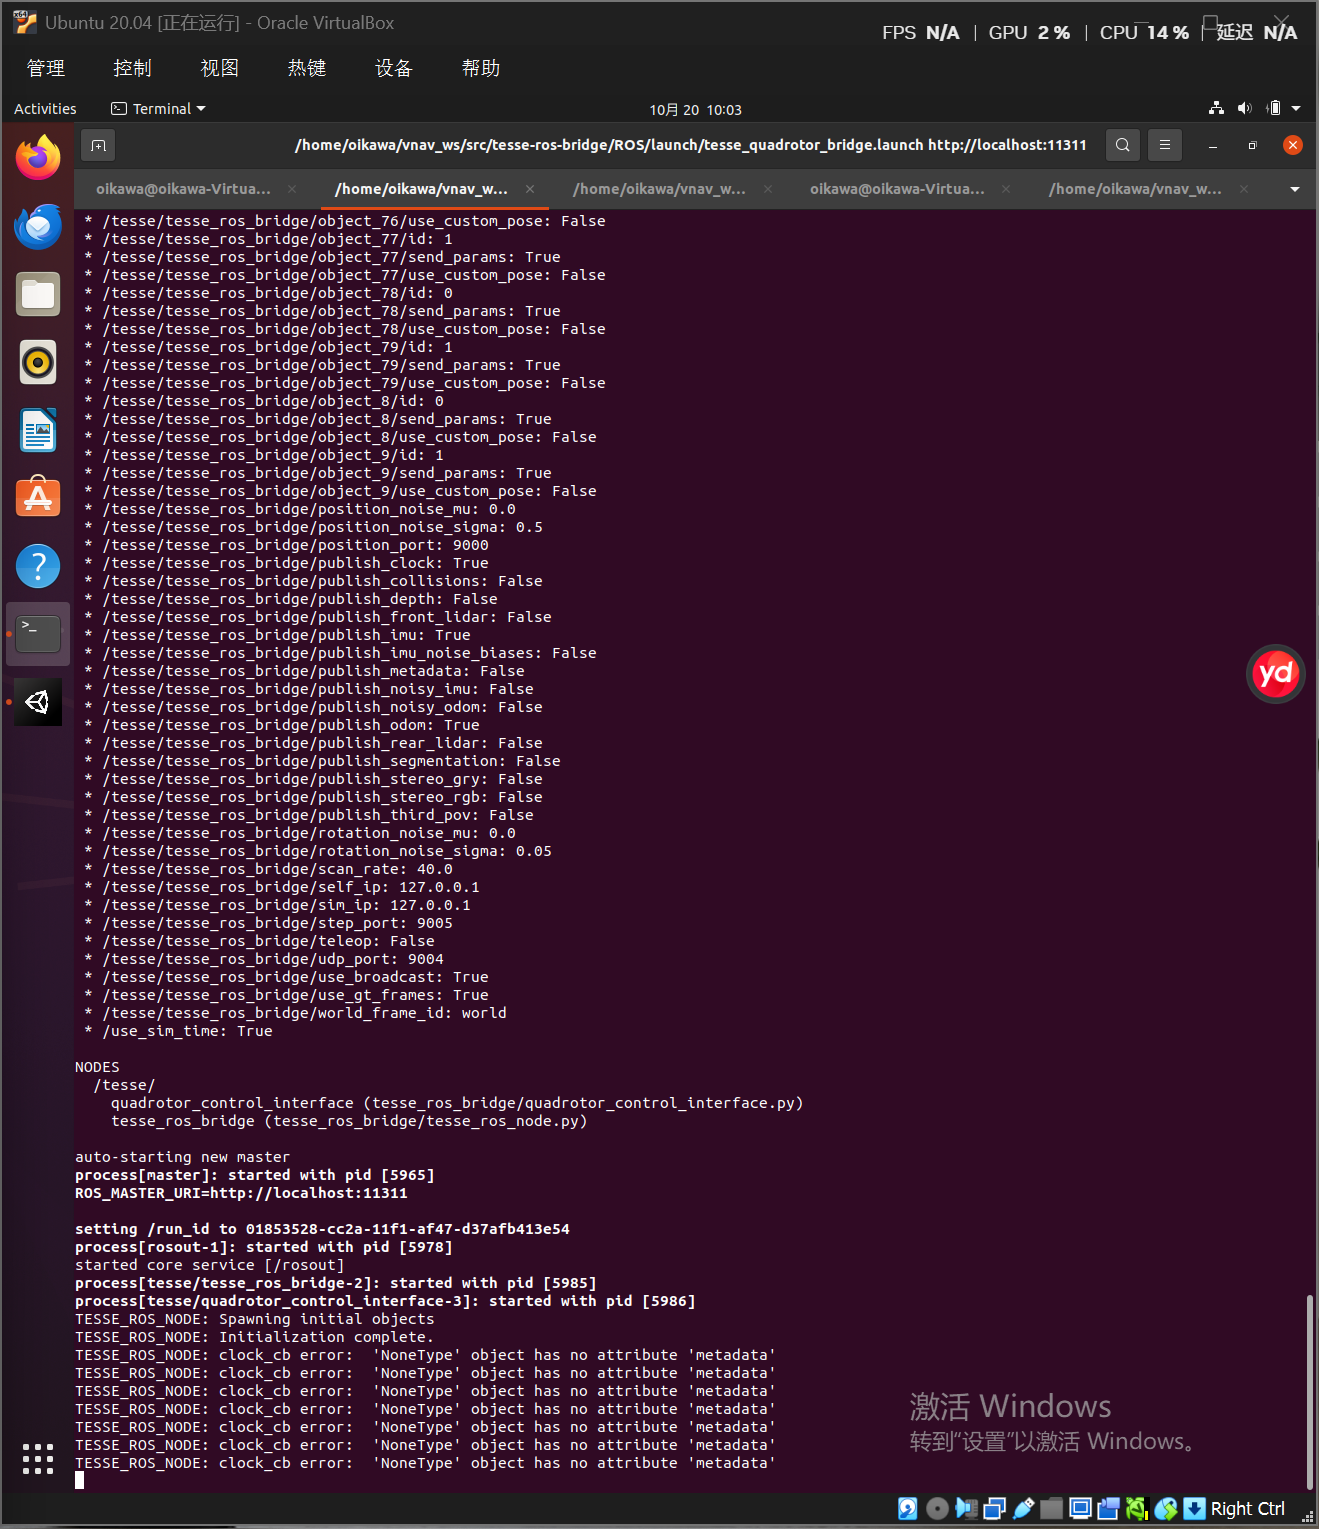
\includegraphics[width=0.94\columnwidth]{fig02_bridge.png}
\caption{TESSE ROS bridge startup and communication parameters.}
\label{fig:bridge}
\end{figure}

\subsection{Trajectory Follower and Waypoint Publisher}
The remaining nodes were launched in order:
\begin{lstlisting}[language=bash]
# Terminal 3
source ~/vnav_ws/devel/setup.bash
roslaunch trajectory_generation traj_following.launch
# Terminal 4
source ~/vnav_ws/devel/setup.bash
roslaunch planner_pkg traj_gen.launch
\end{lstlisting}
The follower starts the optimizer and controller, then waits for waypoints. Launching \texttt{traj\_gen.launch} publishes the course poses, triggers trajectory generation, and begins desired-state publication. Figure~\ref{fig:waypointlaunch} shows the waypoint publisher launched after the simulator, bridge, and follower.

\begin{figure}[!htbp]
\centering
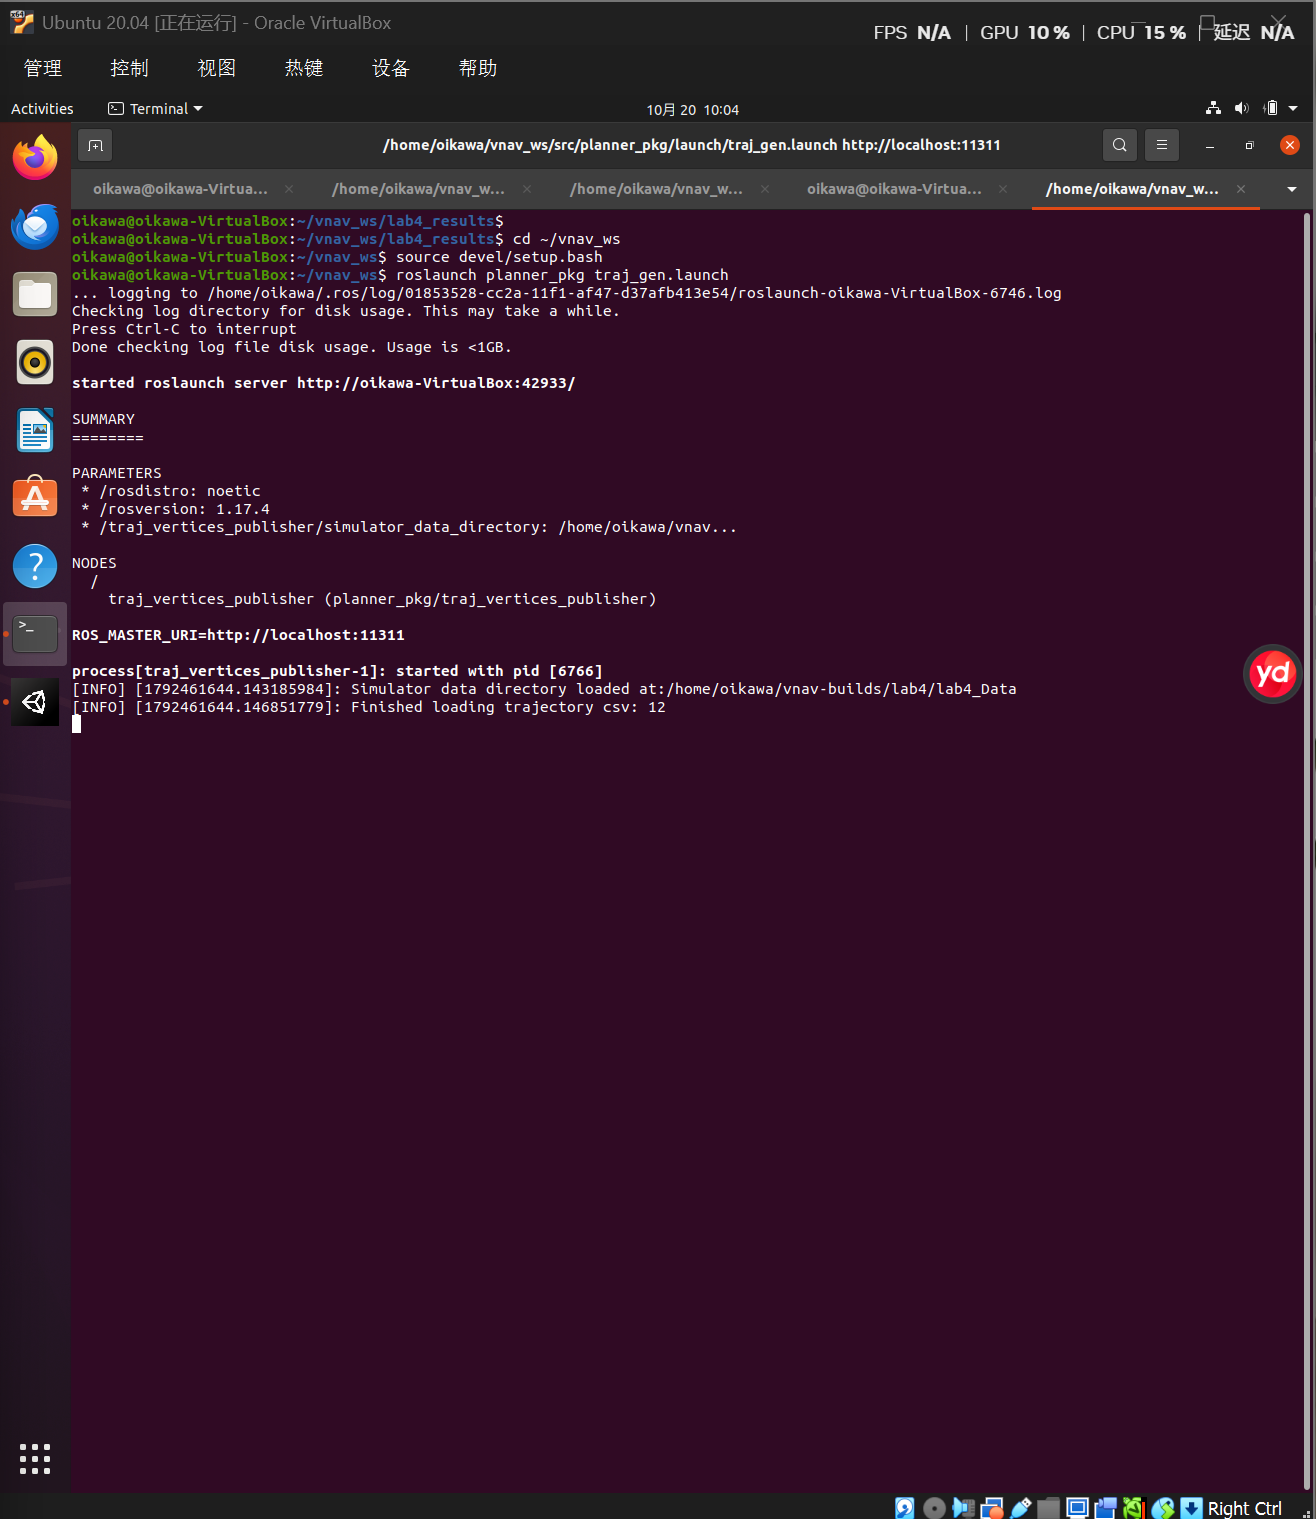
\includegraphics[width=0.94\columnwidth]{fig05_waypoint_launch.png}
\caption{Waypoint publisher launched after the simulator bridge and trajectory follower.}
\label{fig:waypointlaunch}
\end{figure}

\section{Experimental Results and Analysis}
\subsection{Trajectory Execution}
During flight, the trajectory node reported the percentage of the sampled duration. Reaching 100\% confirms that the sampling time advanced to the end of the generated trajectory; course completion must additionally be checked in Unity.

\begin{figure}[!htbp]
\centering
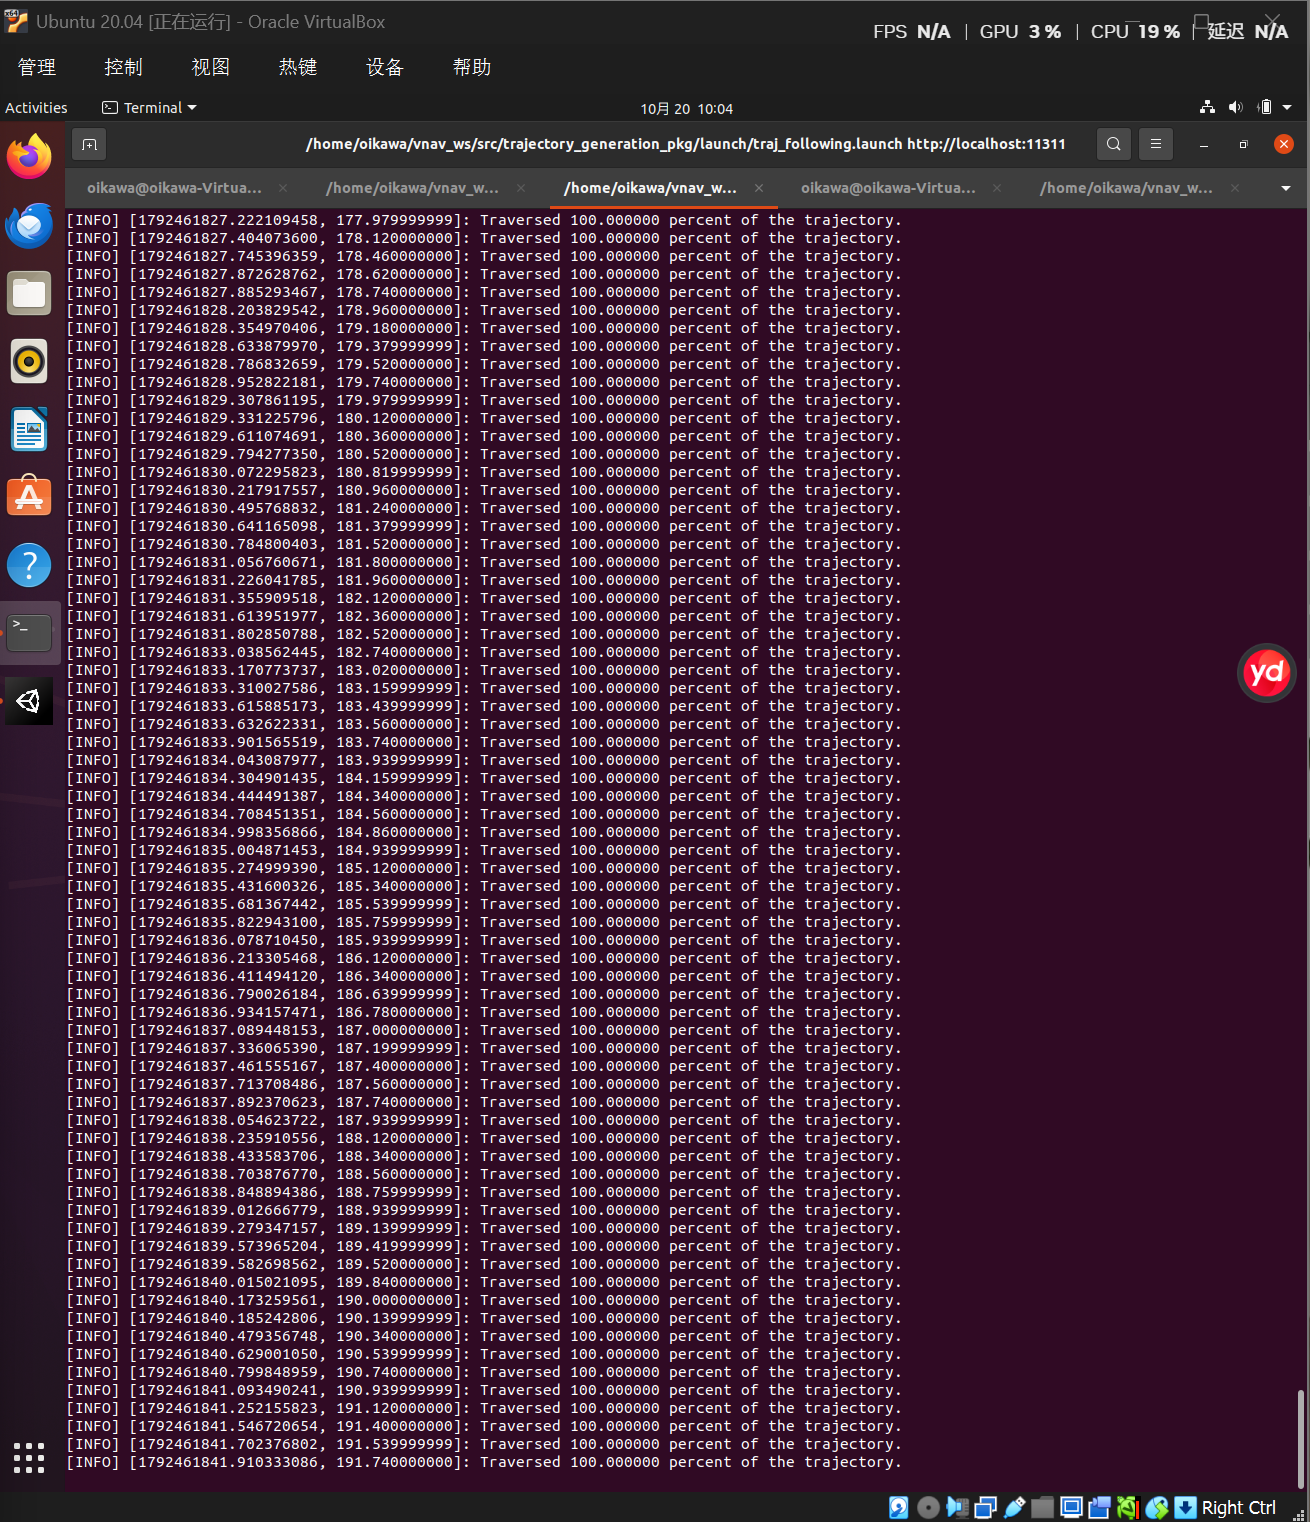
\includegraphics[width=0.94\columnwidth]{fig10_trajectory_100.png}
\caption{Trajectory follower reporting 100\% traversal of the generated reference.}
\label{fig:progress}
\end{figure}

The baseline run showed the UAV following the optimized reference through the course. The final Unity view confirms arrival at the latter part of the track and successful completion of the available baseline run.

\begin{figure}[!htbp]
\centering
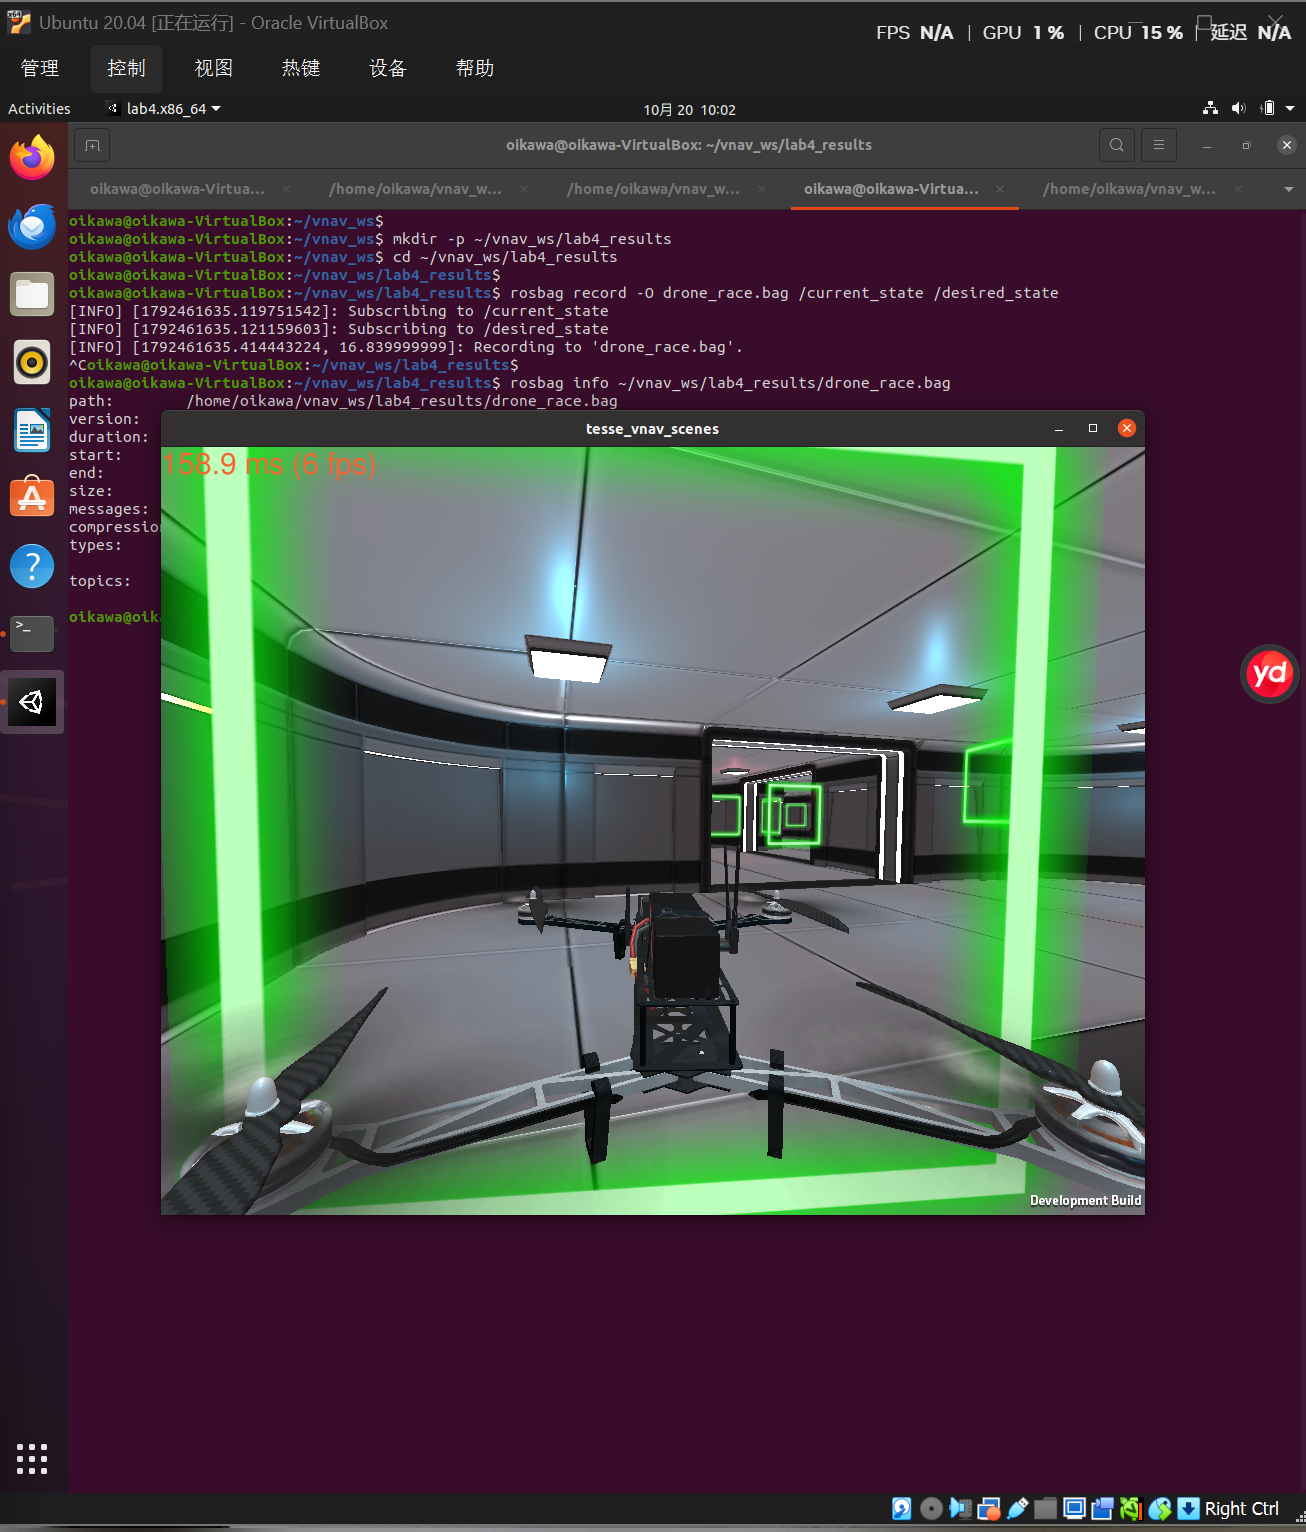
\includegraphics[width=0.94\columnwidth]{fig11_race_complete.png}
\caption{Successful completion of the baseline Unity drone-racing course.}
\label{fig:complete}
\end{figure}

The verified module-level results are summarized in Table~\ref{tab:results}.
\begin{table}[!htbp]
\caption{Functional Verification Results}
\label{tab:results}
\centering
\footnotesize
\begin{tabular}{@{}p{0.58\columnwidth}p{0.30\columnwidth}@{}}
\toprule
Module or check & Result\\
\midrule
ROS-Unity communication & Operational\\
Gate-pose publication & Operational\\
Position/yaw constraint construction & Operational\\
Minimum-snap solution & Operational\\
Desired-state publication & Operational\\
Controller trajectory tracking & Verified\\
Baseline complete flight & Completed\\
Fastest-run quantitative comparison & Pending\\
\bottomrule
\end{tabular}
\end{table}

\subsection{Trajectory Data Recording Procedure}
To compare measured and desired trajectories, \texttt{/current\_state} and \texttt{/desired\_state} should be recorded before the waypoint publisher is launched:
\begin{lstlisting}[language=bash]
mkdir -p ~/vnav_ws/lab4_results
cd ~/vnav_ws/lab4_results
rosbag record -O drone_race_final.bag \
  /current_state /desired_state
\end{lstlisting}
After the complete flight, \texttt{Ctrl+C} closes the recording cleanly, and
\begin{lstlisting}[language=bash]
rosbag info ~/vnav_ws/lab4_results/drone_race_final.bag
\end{lstlisting}
verifies the contained topics. The available screenshot confirms that both required topics were captured, but the final fastest-run bag and its public submission link remain to be supplied with the team result. No recording duration is interpreted as a race time.

\begin{figure}[!htbp]
\centering
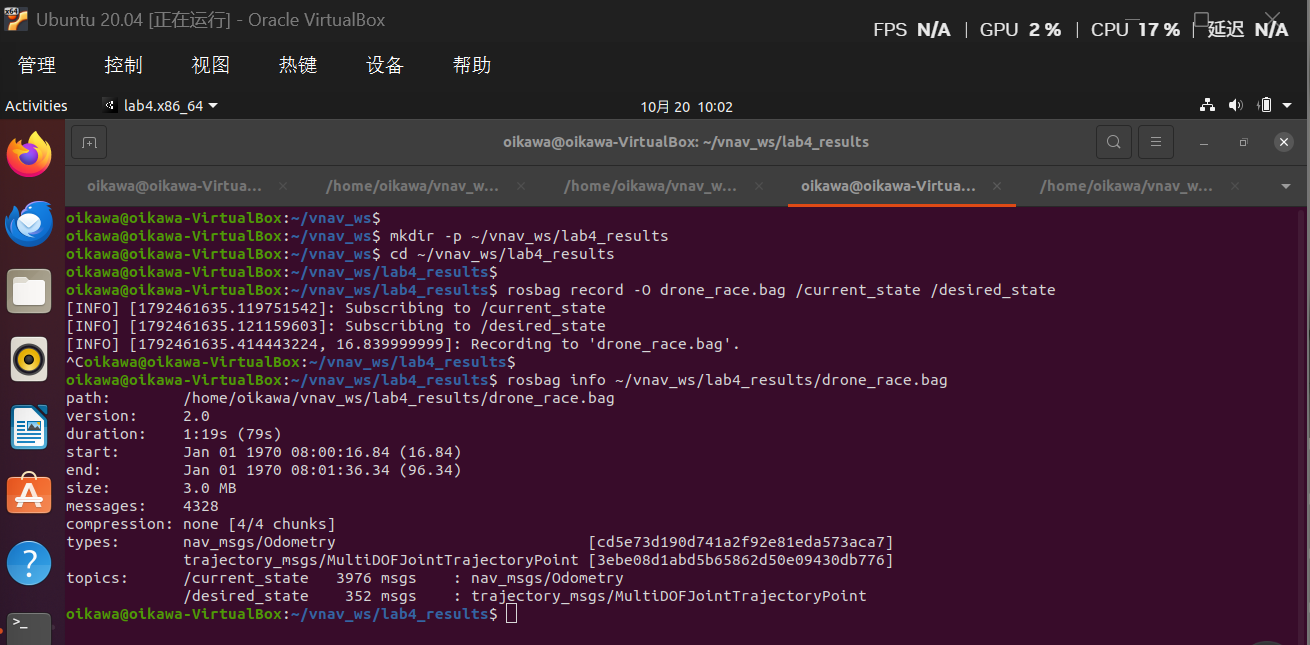
\includegraphics[width=0.98\columnwidth]{fig12_rosbag.png}
\caption{Preliminary rosbag topic verification for current and desired states.}
\label{fig:rosbag}
\end{figure}

\subsection{Final Team Submission Status}
The course requires a video of the complete race and a rosbag from the complete fastest run. Both files must be uploaded to a publicly viewable location, and their links must be placed in \texttt{rviz\_drone\_race.txt}. At the time of writing, the teammate is still adjusting the final race video and speed parameters. Therefore, the baseline completion is documented, but no final fastest time or optimized-versus-baseline numerical comparison is claimed.

\section{Problems Encountered and Solutions}
\subsection{Startup Synchronization}
Repeated bridge \texttt{clock\_cb} messages indicated that metadata was not immediately available. The system later recovered and completed the hover and race. The practical solution is to wait for the Unity scene to finish loading before launching the bridge; if the error persists, restart Unity and the related ROS nodes.

\subsection{Resetting a Race}
Pressing \texttt{r} in Unity resets the vehicle pose but does not necessarily reset the optimized trajectory, ROS start time, or cached node state. A reliable rerun therefore uses the following sequence: stop the current launch processes, close and restart Unity, restart the bridge, restart the trajectory follower, and launch the waypoint publisher last. This prevents a new vehicle state from being paired with an old trajectory clock.

\subsection{Build Warnings and Functional Verification}
The \texttt{\%d}/\texttt{size\_t} warning should be corrected with \texttt{\%zu}, and stale backup files should be removed before repository submission. More importantly, a successful build is not sufficient evidence of functional completeness. The experiment therefore combined source inspection, topic checks, first-gate hovering, trajectory progress, and the final Unity view.

\subsection{Speed, Stability, and Measurement Limits}
Increasing $v_{\max}$ or $a_{\max}$ reduces estimated segment times but may increase tracking error and controller effort. The present results validate the baseline configuration; they do not establish the fastest stable configuration. Future analysis should align \texttt{/current\_state} and \texttt{/desired\_state}, compute peak and root-mean-square position errors, record gate-wise clearance, and measure race time independently. Such metrics would distinguish a genuinely faster and accurate trajectory from a reference that merely advances more quickly.

\section{Conclusion}
This experiment connected analytical trajectory optimization to a complete autonomous drone-racing implementation. The individual derivation showed that increasing polynomial degree does not reduce the minimum-velocity cost under position-only endpoint constraints, while an added terminal-velocity condition makes the cubic solution beneficial. The multi-segment analysis established the polynomial degree and constraint count for minimum snap and the general minimum-$r$th-derivative case.

On the implementation side, the Lab 3 controller was integrated with consistent gains; the first-gate hover was verified; current position was extracted from odometry; gate poses were converted into position and continuous-yaw constraints; position and yaw minimum-snap trajectories were solved; and complete desired states were published periodically. Source checks and the successful build of all 20 packages were followed by Unity validation of the baseline course. The remaining team work is to finalize speed tuning, record the fastest complete run, upload its video and rosbag, and add both public links to \texttt{rviz\_drone\_race.txt}.

\begin{thebibliography}{99}
\bibitem{mitlab4}
MIT 16.485 Visual Navigation for Autonomous Vehicles, ``Lab 4: Trajectory Optimization and Drone Racing,'' 2023.
\bibitem{mittrajnotes}
MIT 16.485 Visual Navigation for Autonomous Vehicles, ``Lecture 9: Trajectory Optimization I,'' Fall 2020.
\bibitem{mellinger2011}
D. Mellinger and V. Kumar, ``Minimum Snap Trajectory Generation and Control for Quadrotors,'' in \emph{Proc. IEEE Int. Conf. Robotics and Automation}, 2011, pp. 2520--2525.
\bibitem{richter2016}
C. Richter, A. Bry, and N. Roy, ``Polynomial Trajectory Planning for Aggressive Quadrotor Flight in Dense Indoor Environments,'' in \emph{Robotics Research}, Springer, 2016, pp. 649--666.
\bibitem{lee2010}
T. Lee, M. Leok, and N. H. McClamroch, ``Geometric Tracking Control of a Quadrotor UAV on SE(3),'' in \emph{Proc. IEEE Conf. Decision and Control}, 2010, pp. 5420--5425.
\bibitem{mavtrajectory}
ETH Zurich Autonomous Systems Lab, ``mav\_trajectory\_generation source package and examples,'' version included with the Lab 4 workspace.
\bibitem{rosmessages}
ROS Noetic, ``Message definitions for nav\_msgs/Odometry and trajectory\_msgs/MultiDOFJointTrajectoryPoint.''
\end{thebibliography}

\end{document}

